\documentclass{diploma}

\student{Алексеев Владислав Евгеньевич}
\group{М8О-406Б-19}
\theme{Разработка базы данных отделения неотложной медицинской помощи с использованием PostgreSQL}

\supervisor{Пивоваров Дмитрий Евгеньевич}
\firstConsultant{---}
\secondConsultant{---}
\reviewer{---}

\faculty{№ 8 <<Компьютерные науки и прикладная математика>>}
\department{806}
\speciality{01.03.02 <<Прикладная математика и информатика>>}
\profile{Информатика}

\departmentFullName{№ 806}
\headOfDepartment{Крылов Сергей Сергеевич}

% Дата. Оставляем пустое место для дня
\date{\uline{\hspace{24pt}} мая \the\year\ года}

\newacronym{БД}{БД}{база данных}
\newacronym{ИС}{ИС}{информационная система}
\newacronym{МКБ}{МКБ}{международная классификация болезней}
\newacronym{НСД}{НСД}{несанкционированный доступ}
\newacronym{ОНМП}{ОНМП}{отделение неотложной медицинской помощи}
\newacronym{ОС}{ОС}{операционная система}
\newacronym{СМП}{СМП}{скорая медицинская помощь}
\newacronym{СУБД}{СУБД}{система управления базами данных}
\newacronym{ACID}{ACID}{атомарность, согласованность, изоляция и долговечность}
\newacronym{ANSI}{ANSI}{американский национальный институт стандартов}
\newacronym{OSI}{OSI}{открытые системы взаимодействия}
\newacronym{TCP}{TCP}{протокол управления передачей}
\newacronym{UDP}{UDP}{протокол пользовтельских датаграмм}
\newacronym{XML}{XML}{расширяемый язык разметки}
\newglossaryentry{id1}{ % Нужны разные id, можно ставить просто последовательно
    name={ACID},
    description={это набор свойств транзакций базы данных, предназначенных для гарантии достоверности данных, несмотря на ошибки, сбои питания и другие неудачи}
}
\newglossaryentry{id2}{
    name={BSON},
    description={это формат электронного обмена цифровыми данными, бинарная форма представления простых структур данных и ассоциативных массивов. Является надмножеством JSON, включая дополнительно регулярные выражения, двоичные данные и даты}
}

\newglossaryentry{id3}{
    name={JSON},
    description={это популярный формат текстовых данных, который используется для обмена данными в современных веб - и мобильных приложениях}
}
\newglossaryentry{id4}{
    name={SQL-инъекция},
    description={это уязвимость, которая позволяет атакующему использовать фрагмент вредоносного кода на языке структурированных запросов (SQL) для манипулирования базой данных и получения доступа к потенциально ценной информации}
}
\newglossaryentry{id5}{
    name={SSL},
    description={это криптографический протокол, который подразумевает более безопасную связь и использует асимметричную криптографию для аутентификации ключей обмена, симметричное шифрование для сохранения конфиденциальности, коды аутентификации сообщений для целостности сообщений}
}
\newglossaryentry{id6}{
    name={TCP},
    description={это важный протокол сети интернет, который позволяет двум хостам создать соединение и обмениваться потоками данных}
}
\newglossaryentry{id7}{
    name={UDP},
    description={это один из ключевых элементов набора сетевых протоколов для Интернета, с помощью которого компьютерные приложения могут посылать сообщения другим хостам по IP-сети без необходимости предварительного сообщения для установки специальных каналов передачи или путей данных}
}
\newglossaryentry{id8}{
    name={Модель OSI},
    description={это сетевая модель стека сетевых протоколов, посредством которой различные сетевые устройства могут взаимодействовать друг с другом}
}
\newglossaryentry{id9}{
    name={Наряд},
    description={это группа медицинских работников и транспортных средств, назначенных для выполнения определенной миссии или задачи, а также медицинское оборудование и инструменты}
}

\addbibresource{main.bib}

% Иллюстрации всегда по центру
\makeatletter
\g@addto@macro\@floatboxreset\centering
\makeatother

\begin{document}
    \maketitle

    % \includepdf[pages=-]{extra/task} % Задание
    \setcounter{page}{2} % Устанавливает счётчик страниц

    \abstract % Структурный элемент: РЕФЕРАТ

 % Реферат

    \tableofcontents % Содержание 
    \termsanddefenitions % Термины и определения
    \listofabbreviations % Перечень сокращений и обозначений
 
    \introduction % Структурный элемент: ВВЕДЕНИЕ

Актуальность темы данной выпускной квалификационной работы бакалавра связана с большим значением проведения эффективных мероприятия по оказанию медицинской помощи пациентам со стороны медицинских работников, максимальное упрощение заполнения документов о выездах и действиях по ее оказанию. Кроме того, врачам иногда требуется некоторый вспомогательный материал в виде информационных данных в таблицах с симптомами диагнозов или дозировками того или иного препарата.

В наше время использование баз данных является одной из неотъемлемых частей работы многих компаний и организаций, так как это позволяет хранить, организовывать и управлять большими объемами данных. Базы данных позволяют быстро и эффективно хранить и обрабатывать данные, что является необходимым условием для принятия важных бизнес-решений.

Одним из наиболее популярных языков для работы с базами данных является PostgreSQL. Он обладает высокой степенью надежности, масштабируемости и производительности. PostgreSQL также поддерживает многие функции, которые делают его удобным для работы с различными типами данных и приложений \cite{book1}.

Использование баз данных также позволяет легко и быстро находить необходимую информацию и управлять ею, а также обеспечивает сохранность и целостность данных, что немаловажно в наших современных реалиях, ведь большинство информации просто напросто может утечь в сеть и оказаться в открытом доступе, желаем мы того или нет. Базы данных позволяют использовать различные методы анализа и обработки данных, что является важным инструментом для повышения эффективности работы компаний и организаций.

Кроме того, использование баз данных является современным и необходимым подходом к работе с данными, который позволяет не только сохранять и управлять ими, но и анализировать и использовать в дальнейшем. Базы данных PostgreSQL являются открытым и свободно распространяемым решением, что делает их доступными и удобными для использования в различных проектах и приложениях.

В современном мире качество медицинской помощи и скорость ее оказания имеют большое значение для общества. Скорая медицинская помощь играет важную роль в сохранении здоровья и жизни людей в случае непредвиденных ситуаций и аварий. Однако, существующая система скорой помощи имеет свои проблемы, связанные с низкой эффективностью и долгим временем ожидания при оказании медицинской помощи.

Внедрение цифровых технологий в работу скорой медицинской помощи может значительно улучшить качество и эффективность ее работы. В частности, организация электронных медицинских карт и использование баз данных на языке PostgreSQL позволят ускорить процесс диагностики и лечения пациентов, а также сократить время ожидания скорой медицинской помощи.

Данная выпускная квалификационная работа имеет практическое значение, так как внедрение цифровых технологий в работу скорой медицинской помощи может ускорить процесс оказания медицинских услуг и повысить их качество, что в свою очередь приведет к улучшению уровня здоровья и жизни населения в целом.

Сейчас врачам важно и нужно переходить на цифровое использование и заполнение медицинских карт при осмотре пациентов по нескольким причинам:

\begin{itemize}
    \item цифровая медицинская карта позволяет быстро и удобно получить доступ к информации о пациенте, что повышает эффективность и точность диагностики и лечения,
    \item цифровая медицинская карта позволяет сохранять и обрабатывать большие объемы данных о пациентах, что является важным инструментом для проведения исследований и разработки новых методов лечения. Также это позволяет врачам получать доступ к общей истории лечения пациента и учитывать его предыдущие заболевания, что повышает качество и эффективность лечения,
    \item использование цифровых медицинских карт позволяет уменьшить вероятность ошибок и искажений при заполнении и хранении информации о пациентах, что обеспечивает сохранность и конфиденциальность медицинских данных.
\end{itemize}

Наконец, использование цифровых медицинских карт является современным и удобным подходом к организации работы медицинских учреждений и обслуживанию пациентов, что способствует повышению уровня медицинской помощи и общей качества жизни населения.

В данной выпускной квалификационной работе бакалавра были использованы различные технологии и инструменты для облегчения исследования, реализации и анализа работы всей системы:

\begin{itemize}
    \item PostgreSQL – мощная реляционная система управления базами данных (СУБД), которая обладает высокой производительностью, масштабируемостью, надежностью и расширяемостью. Она поддерживает широкий спектр функций, позволяет работать с различными типами данных и обеспечивает сохранность и целостность данных,
    \item PgAdmin – это графический инструмент для администрирования баз данных PostgreSQL. Он предоставляет удобный интерфейс для управления базами данных и объектами в них, такими как таблицы, индексы, пользователи и многое другое. PgAdmin поддерживает широкий диапазон функций, включая создание и редактирование объектов базы данных, выполнение SQL-запросов, экспорт и импорт данных, а также управление безопасностью и настройками базы данных,
    \item Erwin – это программное обеспечение для моделирования баз данных. Оно позволяет проектировать их визуально в удобном графическом интерфейсе. Erwin поддерживает множество популярных СУБД, включая PostgreSQL, и предоставляет широкий набор инструментов для работы с базами данных, таких как автоматическое генерирование SQL-кода, проверка целостности данных, анализ производительности и многое другое.
\end{itemize}

С научной точки зрения, данная работа вносит вклад в существующий массив знаний о разработке и проектировании баз данных и их эффективности в различных сценариях нагрузки и использования. С практической точки зрения, данное исследование предоставляет ценные идеи для медицинских работников, для которых так важно оптимизировать свои действия по заполнению медицинских карт, карт осмотра пациентов и многие другие рутинные задачи.

Таким образом, данная выпускная квалификационная работа бакалавра является актуальной и с научно-методической/теоретической, и с практической точек зрения. % Введение

    % Название разделов -- все прописные
\section{ТЕОРЕТИЧЕСКОЕ ОБОСНОВАНИЕ РАЗРАБОТКИ БАЗЫ ДАННЫХ}

\subsection{Анализ предметной области}

Анализ предметной области является первым этапом в проектировании базы данных, в ходе которого выделяются основные объекты и их свойства, определяются первоначальные требования и границы проекта, чтобы разработать эффективную и безопасную базу данных.

Предметной областью разрабатываемой модели данных является система заполнения электронных медицинских карт для отделения неотложной медицинской помощи.

Скорая медицинская помощь (СМП) – вид медицинской помощи, оказываемой гражданам при заболеваниях, несчастных случаях, травмах, отравлениях и других состояниях, требующих срочного медицинского вмешательства.

Отделение неотложной (экстренной) медицинской помощи больницы является структурным подразделением многопрофильной больницы, которое в круглосуточном режиме оказывает экстренную (неотложную) медицинскую помощь.

Медицинская помощь включает в себя процедуру проведения осмотра, непосредственно манипуляции по оказанию медицинской помощи, а также консультирование пациента по с целью определения наиболее эффективного, безопасного и экономически оправданного курса лечения.

ОНМП осуществляет следующие функции:

\begin{itemize}
    \item прием пациентов с острыми заболеваниями, несчастными случаями, травмами, отравлениями и другими состояниями, требующими немедленной медицинской помощи;
    \item проведение первичной медицинской диагностики и оценки состояния пациента, осуществление мер, направленных на стабилизацию состояния пациента;
    \item предоставление неотложной медицинской помощи, включая проведение лечебных манипуляций, инъекций, переливание крови, а также оказание психологической помощи;
    \item организация и координация работы других специалистов и служб в медицинском учреждении, если необходимо;
    \item подготовка пациента к транспортировке в стационар для дальнейшего лечения;
    \item соблюдение всех медицинских стандартов и требований, направленных на обеспечение безопасности пациентов и медицинского персонала;
    \item организация транспортировки пациентов в случае необходимости;
    \item обеспечение работы необходимого медицинского оборудования, инструментов, материалов и медикаментов, необходимых для оказания неотложной медицинской помощи,
    \item проведение медицинской документации, включая учет медицинских случаев, регистрацию историй болезни и медицинских записей;
    \item обеспечение мониторинга и контроля за состоянием пациентов, находящихся на лечении в отделении неотложной (экстренной) медицинской помощи;
    \item обучение медицинского персонала и сотрудников отделения неотложной медицинской помощи новым методам лечения и диагностики;
    \item сотрудничество и консультации с другими медицинскими учреждениями, специалистами и службами для повышения качества оказываемой медицинской помощи.
\end{itemize}

Отделение неотложной (экстренной) медицинской помощи является ключевым звеном в системе оказания медицинской помощи населению и обеспечивает быстрое и эффективное лечение при острых заболеваниях и травмах.

Базы данных для неотложной медицинской помощи являются критически важным элементом в работе современных медицинских учреждений. Они позволяют эффективно организовывать, хранить и обрабатывать медицинскую информацию, ускоряя процессы принятия решений и повышая качество медицинской помощи.

Основным требованием к базе данных для неотложной медицинской помощи является ее способность оперативно и точно хранить медицинскую информацию о пациентах. Эта информация может включать данные о медицинской истории пациента, диагнозе, принятых мероприятиях, результатах обследований и лекарственном лечении.

Для эффективного управления медицинской информацией в базе данных неотложной медицинской помощи необходима специализированная система управления базами данных (СУБД). Существует множество СУБД, которые могут использоваться для этой цели, включая Oracle, MySQL, Microsoft SQL Server, PostgreSQL и др.

Также необходимо учитывать специфику работы медицинских учреждений, которые могут иметь различные требования к хранению и обработке медицинской информации. Например, больницы могут иметь разные отделения, каждое из которых может иметь свои особенности в обработке информации. Кроме того, необходимо учитывать возможность интеграции с другими системами, такими как системы управления ресурсами и планирования процессов.

Важно также отметить, что база данных для неотложной медицинской помощи должна соответствовать требованиям законодательства в области защиты персональных данных, таких как Федеральный закон от 27 июля 2006 года № 152-ФЗ «О персональных данных». Регулярное обновление и адаптация базы данных к изменениям в законодательстве помогут поддерживать соответствие нормам и предотвращать правовые проблемы.

Исследования показывают, что эффективное использование баз данных в медицинских учреждениях может значительно улучшить качество медицинской помощи и снизить затраты на ее оказание. Например, использование баз данных может уменьшить количество ошибок в принятии решений, сократить время, необходимое для оказания медицинской помощи, и повысить точность диагностики.

На текущий момент существует множество различных подходов к проектированию баз данных для медицинских учреждений. Некоторые из них ориентированы на сохранение структурированной информации, другие на работу с полуструктурированными и неструктурированными данными.

Одним из наиболее распространенных подходов к проектированию баз данных для медицинских учреждений является использование реляционной модели данных \cite{book6}. Реляционная модель данных позволяет хранить информацию в виде таблиц, которые могут быть связаны друг с другом через ключи. Это позволяет обрабатывать большие объемы структурированных данных и осуществлять запросы на выборку данных, используя язык SQL.

Тем не менее, в последние годы набирают популярность нереляционные базы данных, такие как MongoDB, Cassandra, Couchbase и др. Они хранят данные в более гибкой форме, позволяют более легко масштабировать базы данных и работать с полуструктурированными и неструктурированными данными, такими как тексты медицинских записей, изображения и видео.

Важным аспектом разработки баз данных для медицинских учреждений является также обеспечение защиты медицинской информации от несанкционированного доступа. Для этого применяются различные меры безопасности, такие как шифрование данных, многофакторная аутентификация и разграничение прав доступа к информации в зависимости от роли пользователя.

Наконец, важно отметить, что разработка баз данных для медицинских учреждений является сложным и многогранным процессом, требующим учета множества факторов, таких как специфика медицинских процедур, законодательство, требования к безопасности и другие. Поэтому необходимо проводить тщательный анализ предметной области и разрабатывать индивидуальные решения для каждого конкретного медицинского учреждения.




\subsection{Анализ существующих подходов}

Перед тем как начинать разработку базы данных, нужно выяснить, какие виды БД существуют, проанализировать их и уже на основе этого делать выводы о наиболее подходящем виде под наши конкретные требования.

Существует несколько видов баз данных, каждый из которых имеет свои особенности и применения:

\begin{itemize}
    \item реляционные базы данных (РБД): это самый распространенный тип БД. В РБД данные организованы в виде таблиц, состоящих из строк (записей) и столбцов (полей). Реляционные БД используют структурированный язык запросов, такой как SQL, для управления данными и выполнения операций, таких как вставка, обновление, удаление и извлечение данных. Примеры реляционных БД включают MySQL, PostgreSQL и Oracle;
    \item иерархические базы данных: в таких БД данные организованы в виде иерархической структуры, состоящей из уровней и подуровней. Каждый уровень может иметь только одного родителя, что создает иерархию. Этот тип БД широко использовался в прошлом, но в настоящее время его применение ограничено. Примеры иерархических БД включают IBM's Information Management System (IMS);
    \item сетевые базы данных: этот тип БД организован в виде сети связанных записей. Записи могут иметь несколько родителей и несколько дочерних записей, что позволяет создавать сложные связи между данными. Сетевые БД также имеют ограниченное применение в настоящее время. Примером сетевой БД является Integrated Data Store (IDS);
    \item объектно-ориентированные базы данных (ООБД): в ООБД данные организованы в виде объектов, которые могут содержать свойства (поля) и методы (функции). ООБД позволяют более натуральное представление сложных структур данных и поддерживают наследование и полиморфизм. Примеры ООБД включают MongoDB и Couchbase;
    \item ключ-значение базы данных: в таких БД данные хранятся в виде пар ключ-значение. Они просты и эффективны для хранения и извлечения данных, но ограничены по функциональности. Примеры ключ-значение БД включают Redis и Apache Cassandra;
    \item документоориентированные базы данных: в этом типе БД данные организованы в виде документов, обычно в формате JSON или XML. Документы могут содержать различные поля и вкладываться друг в друга, образуя более сложную структуру;
    \item временные базы данных: эти базы данных предназначены для хранения и управления временными данными, такими как временные ряды, события и временные маркировки. Они оптимизированы для выполнения операций, связанных с временными данными, такими как агрегация, интерполяция и анализ трендов. Примеры временных баз данных включают InfluxDB и TimescaleDB;
    \item массивные параллельные обработки (MPP) базы данных: эти базы данных разработаны для обработки больших объемов данных с использованием параллельных вычислений на распределенных системах. Они позволяют выполнить параллельную обработку запросов и аналитики на большом количестве узлов. Примеры MPP БД включают Amazon Redshift и Google BigQuery.
\end{itemize}
    
Каждый из этих видов БД предназначен для решения определенных задач и имеет свои преимущества и ограничения. Выбор типа базы данных зависит от конкретных требований проекта, характеристик данных и ожидаемой производительности.

После того, как были рассмотрены различные виды БД, приведем существующие аналоги предполагаемой разработки. На данный момент существует несколько общеизвестных баз данных для отделений неотложной медицинской помощи:

\begin{itemize}
    \item федеральная медицинская информационная система (ФМИС): ФМИС является единым информационным ресурсом для системы здравоохранения в России. Она объединяет различные базы данных и модули, включая модуль неотложной медицинской помощи. В рамках этой системы регистрируются и хранятся данные о поступающих в отделения неотложной помощи пациентах. В ФМИС включены сведения о пациентах, результаты обследований и лечения, информация о медицинских событиях;
    \item единая автоматизированная информационная система "Амбулатория": эта система разработана для работы с амбулаторными картами пациентов и учета медицинской информации. Она может быть использована в поликлиниках и отделениях неотложной помощи. В рамках системы "Амбулатория" регистрируются пациенты, ведется электронная история болезни, хранятся результаты обследований и лечения. Система также позволяет врачам планировать визиты, назначать лекарства и процедуры, а также отслеживать текущее состояние пациента;
    \item система учета вызовов скорой медицинской помощи (СУВ): эта система предназначена для приема и учета вызовов скорой помощи. Она используется диспетчерскими службами скорой помощи для регистрации информации о вызывающем лице, месте происшествия, описании ситуации и оценке состояния пациента. СУВ позволяет оперативно отправлять бригады скорой помощи на место происшествия и отслеживать их движение в реальном времени. В системе также регистрируются данные о времени прибытия бригады, оказанной помощи и транспортировке пациента;
    \item информационная система "Регистр оказания скорой медицинской помощи" (РОСМЕД): эта система используется для сбора и анализа данных о оказании скорой медицинской помощи в России. РОСМЕД предназначена для регистрации информации о вызовах скорой помощи, диагнозах, примененных медицинских манипуляциях и результатах оказания помощи. В систему вносятся данные о каждом вызове скорой помощи, включая информацию о времени вызова, причине вызова, медицинских мерах, принятых бригадой скорой помощи, а также о результате лечения или транспортировке пациента.
\end{itemize}

Эти базы данных - ФМИС, система "Амбулатория", СУВ и РОСМЕД - представляют собой информационные системы, используемые в различных аспектах медицинской помощи в России. Они помогают в сборе, хранении и управлении медицинской информацией, что способствует более эффективному и качественному оказанию неотложной медицинской помощи пациентам.

Все существующие БД хорошо выполняют свой спектр функций, но ни одна из рассмотренных систем не дает автоматизации и упрощения работы медицинского работника непосредственно во время вызова. Работнику все равно приходится работать с бумажными носителями и заполнять все вручную, а лишь потом происходит оцифровка всех собранных данных о пациенте.

Наша же задача стоит в том, чтобы организовать весь спектр проводимых манипуляций с информацией от момента вызова, до момента возвращения бригады в ОНМП в электронном виде для ускорения работ и минимизации ошибок при заполнении медицинских карт, выставлении диагноза и оказания требуемой медицинской помощи.




\subsection{Назначение и возможности базы данных}

В предметной области системы заполнения электронных медицинских карт для отделения неотложной медицинской помощи, основные объекты и свойства, которые следует рассмотреть, могут включать:

\begin{itemize}
    \item пациенты: информация о каждом пациенте, включая персональные данные (имя, дата рождения, пол и контактная информация), медицинскую историю, диагнозы, принятые мероприятия, результаты обследований и лекарственное лечение;
    \item медицинские работники: данные о врачах, медсестрах и других медицинских специалистах, включая их идентификационные данные, специализацию, график работы и доступные привилегии;
    \item медицинские процедуры: информация о проводимых процедурах, включая коды процедур, описания, стоимость, требуемое оборудование и прочие детали;
    \item отделения: данные о различных отделениях неотложной медицинской помощи в больнице, их назначение, доступный персонал и оборудование;
    \item ресурсы: информация о доступных ресурсах, таких как медицинское оборудование, лекарства, материалы и другие необходимые средства;
    \item расписание: график работы медицинского персонала и расписание доступности отделений и ресурсов;
    \item системы управления и интеграция: необходимо учесть возможность интеграции с другими системами, такими как системы управления ресурсами и планирования процессов, чтобы обеспечить эффективное взаимодействие и координацию деятельности медицинских учреждений.
\end{itemize}

Для лучшего понимания предметной области, рассмотрим конкретный пример - разработку базы данных для отделения неотложной медицинской помощи.

Медицинские работники оказывают медицинскую помощь пациентам с острыми заболеваниями и травмами, которые требуют немедленного вмешательства, также необходимо быстро и точно определить диагноз, назначить лечение и принять меры по сохранению жизни пациента.

Одной из основных задач базы данных для отделения неотложной медицинской помощи является хранение и обработка медицинских данных пациентов, включая информацию о симптомах, диагнозах, назначенных лекарствах, процедурах и т.д. Кроме того, необходимо учитывать, что пациенты могут обращаться за медицинской помощью в нескольких отделениях неотложной медицинской помощи, поэтому база данных должна позволять обмениваться информацией между различными медицинскими учреждениями.

Для решения этих задач можно использовать реляционную базу данных, в которой каждый пациент будет представлен в виде отдельной записи в таблице, содержащей данные о пациенте, диагнозах, лекарствах и т.д. Ключами в таблицах могут быть номера пациента, номера записи и т.д. Это позволит производить выборку данных о конкретном пациенте, обращаться к истории его болезни, проводить анализ данных и выявлять тенденции в заболеваемости и лечении.

Однако, реляционная модель может столкнуться с проблемами при работе с полуструктурированными и неструктурированными данными, такими как медицинские изображения, видео и тексты медицинских записей. Для работы с этими данными может использоваться нереляционная база данных, такая как MongoDB. В MongoDB данные могут быть храниться в более гибкой форме, используя форматы, такие как JSON и BSON. MongoDB также позволяет хранить и обрабатывать файлы в формате BLOB (binary large object), что делает его идеальным инструментом для хранения медицинских изображений и других неструктурированных данных.

Еще одной важной задачей при разработке базы данных для отделения неотложной медицинской помощи является обеспечение безопасности хранения и доступа к медицинским данным. Для этого может использоваться различные меры, такие как шифрование данных, авторизация пользователей и аудит доступа.

Также при проектировании базы данных для отделения неотложной медицинской помощи необходимо учитывать требования к ее масштабируемости, отказоустойчивости и производительности. В случае большого количества пациентов и медицинских записей может потребоваться использование кластерной архитектуры, репликации данных и других технологий, позволяющих обеспечить высокую доступность и производительность базы данных. Также необходимо обрабатывать большие объемы данных и поддерживать быстрый доступ к ним \cite{online14}.

На сегодняшний день существует множество различных систем управления базами данных, которые могут быть использованы для разработки базы данных для отделения неотложной медицинской помощи, включая MySQL, PostgreSQL, Oracle Database, Microsoft SQL Server, MongoDB и др. Выбор конкретной системы управления базами данных зависит от требований к производительности, масштабируемости, отказоустойчивости и других факторов.

Анализируя все вышеперечисленные требования к организации базы данных, можно сделать вывод, что основным субъектом данной базы данных является врач, который будет осуществлять выезд и непосредственное оказание всех необходимых медицинских услуг.

Врач может иметь доступ к данным о препаратах, находящихся в использовании у данного наряда, он может осуществить поиск по названию лекарственного средства для оперативного предоставления ответа по запросу клиента.

Основные реализуемые функции:
\begin{itemize}
    \item аутентификация и авторизация;
    \item разграничение ролей пользователей;
    \item добавление и удаление данных;
    \item поиск данных по нескольким критериям;
    \item вывод вспомогательных информационных таблиц.
\end{itemize}

\bigbreak
\textbf{Выводы по разделу}
\bigbreak

Проектирование базы данных для системы заполнения электронных медицинских карт является сложным процессом, требующим тщательного анализа предметной области, определения требований и границ проекта, выбора подходящей модели данных и СУБД, обеспечения безопасности данных, обучения пользователей и поддержки системы. Это комплексный процесс, который должен выполняться с участием экспертов в области медицины и баз данных для достижения оптимального результата. Результатом успешной разработки будет эффективная система управления медицинской информацией, способствующая повышению качества медицинской помощи, оптимизации процессов и улучшению результатов лечения пациентов.

В конечном итоге, разработка базы данных для отделения неотложной медицинской помощи является сложной задачей, которая требует учета множества факторов, таких как безопасность, масштабируемость, отказоустойчивость и производительность. Решение этих задач требует использование различных технологий и систем управления базами данных, а также тщательного анализа требований и потребностей пользователей. % Основная часть
    \section{ПРОЕКТИРОВАНИЕ И РАЗРАБОТКА БАЗЫ ДАННЫХ}

\subsection{Выбор программных средств для реализации базы данных}

Выбор программных средств играет большое значение для проектируемой базы данных, поскольку определенные на этом этапе программные продукты, средства разработки и технологии непосредственным образом окажут влияние на распространение разработанной продукта: чем более распространенными будут используемые при разработке и требуемые для функционирования базы данных технологии, тем шире круг потенциальных потребителей, имеющих возможность ей воспользоваться. Кроме того, выбор среды разработки непосредственно влияет на стоимость и простоту процесса разработки в целом.

База данных «onmp» является реляционной. Реляционная база данных представляет собой набор таблиц, однако достаточно часто в состав базы данных входят и другие элементы, позволяющие дополнительно влиять на организацию и структуру данных в соответствии с определенным набором требований.

Создание и развитие динамических веб-страниц требует использования различных технологий. Разработка динамических веб-страниц включает три основных компонента: веб-сервер, язык программирования сценариев, исполняемых на стороне сервера, и базу данных.

Язык структурированных запросов (Structured Query Language, SQL) – самый распространенный язык, предназначенный для записи, извлечения, обновления и удаления информации в системах управления реляционными базами данных.

PostgreSQL (полное название «PostgreSQL: The world's most advanced open source relational database») - это мощная объектно-реляционная система управления базами данных (СУБД), которая поддерживает SQL-запросы и соответствует многим стандартам ANSI SQL. PostgreSQL является свободным и открытым программным обеспечением, доступным для использования и модификации бесплатно.

PostgreSQL обладает рядом преимуществ по сравнению с другими СУБД \cite{book2, book3} :

\begin{itemize}
    \item надежность и целостность данных: PostgreSQL имеет высокую степень надежности и обеспечивает высокую степень целостности данных благодаря поддержке транзакций, атомарности, согласованности и изоляции (ACID);
    \item безопасность: PostgreSQL обеспечивает множество функций безопасности, включая возможность управления правами доступа на уровне таблиц, столбцов, функций и процедур, проверку подлинности и защиту от SQL-инъекций;
    \item масштабируемость: PostgreSQL обладает высокой степенью масштабируемости и может обрабатывать большие объемы данных. Он поддерживает репликацию данных и многоуровневую архитектуру серверов;
    \item поддержка SQL: PostgreSQL поддерживает стандарт SQL и соответствует многим стандартам ANSI SQL, что облегчает разработку и поддержку приложений;
    \item расширяемость: PostgreSQL поддерживает расширения, которые позволяют разработчикам создавать свои собственные функции, типы данных и языки программирования, расширяя тем самым функциональность базы данных;
    \item мощный функционал: PostgreSQL имеет широкий функционал, включая поддержку полнотекстового поиска, гео-пространственных запросов, JSON- и XML-обработки, а также многопоточности;
    \item открытость: PostgreSQL является свободным и открытым программным обеспечением, доступным для использования и модификации бесплатно, что обеспечивает независимость от поставщика и поддержку со стороны большого сообщества разработчиков и пользователей.
\end{itemize}



\subsection{Проектирование базы данных}

Проектирование базы данных для любой автоматизированной системы разделяется на следующие этапы \cite{book5}:

\begin{itemize}
    \item определение требований к базе данных;
    \item концептуальное проектирование базы данных;
    \item выбор средств реализации базы данных;
    \item логическое проектирование;
    \item физическое проектирование.
\end{itemize}

Объекты, которые хранятся в базе данных, имеют некую логическую структуру, то есть описываются некоторой моделью представления данных. К числу классических моделей относят следующие: иерархическая, сетевая и реляционная.

Иерархическая модель представляет собой упорядоченную совокупность данных, организованных в виде дерева, где каждый узел содержит записи данных. Тип «дерево» является составным, состоящим из подтипов (поддеревьев), которые также являются типом "дерево". Каждый тип "дерево" состоит из одного корневого типа и упорядоченного набора подчиненных типов, устанавливая связь «предок-потомок».

Сетевая модель отображает различные взаимосвязи данных в произвольном графе и обобщает иерархическую модель данных. Она использует два типа данных: записи и связи. Связь определяется между двумя типами записей - предком и потомком. В отличие от иерархической модели, где потомок имеет только одного предка, здесь потомок может иметь произвольное число предков.

Реляционная модель основывается на понятии отношений и представляет собой множество элементов, называемых кортежами. Отношение часто представляется в виде двумерной таблицы. Каждая строка таблицы имеет одинаковую структуру и состоит из полей. Строкам соответствуют кортежи, а столбцам - атрибуты. Реляционная модель удобна для описания простых связей между объектами, где каждому объекту соответствует строка таблицы. Если требуется описать более сложные логические структуры данных, часто используют связывание нескольких таблиц.

Для реализации данной медицинской информационной системы будем использовать реляционную модель.

Концептуальная модель базы данных - это наглядная диаграмма, которая использует стандартные обозначения и детально показывает связи между объектами и их характеристиками. Концептуальная модель создается для последующего проектирования базы данных и ее преобразования, например, в реляционную базу данных. В концептуальной модели визуально отображаются связи между объектами данных и их характеристиками \cite{online4}.

ER-модель – модель данных, позволяющая описывать концептуальные схемы на основе диаграмм сущность-связь (ER-диаграмм).

Модель базы данных описывают с помощью одной или нескольких ER- диаграмм, содержащих сущности, атрибуты и связи.

Сущность определяется как объект, событие или концепция, информация о котором должна сохраниться. Сущности имеют наименование, несущее четкое смысловое значение. Каждый экземпляр сущности на диаграмме уникален.

Атрибут хранит информацию об определенном свойстве сущности и имеет четкое смысловое значение. Атрибут или группа атрибутов, которые однозначно идентифицируют экземпляры сущности, называются первичным ключом (англ. primary key).

Связь описывает логическое соотношение между сущностями. Связь сущности с другими сущностями определяет ее тип: различают два типа сущностей – зависимые и независимые.

Можно установить следующие связи между сущностями: идентифицирующая связь «Один–ко–Многим», связь «Многие–ко–Многим», неидентифицирующая связь «Один–ко–Многим» и связь «Один–к–Одному».

Связь «Многие–ко–Многим» существует только на логическом уровне. При переходе на физический уровень это отношение должно быть преобразовано за счет добавления новой зависимой сущности, связанной идентифицирующими связями «Один–ко–Многим» с сущностями, находящимися в исходном отношении.

Сущности, имеющие связь «Один–к–Одному», можно объединить в одну. При физической реализации базы данных две таблицы могут использоваться вместо одной по соображениям конфиденциальности, для удобства, для экономии дискового пространства, из семантических соображений.

Идентифицирующая связь устанавливается между независимой и зависимой сущностями, при этом зависимая сущность не может существовать самостоятельно - экземпляр зависимой сущности определяется только через отношение к сущности, которая его идентифицирует. При установлении идентифицирующей связи атрибуты первичного ключа родительской сущности автоматически переносятся в состав ключевых атрибутов дочерней сущности.  В дочерней сущности новые атрибуты помечаются как внешний ключ. В случае неидентифицирующей связи внешний ключ не входит в состав первичного ключа дочерней сущности.



\subsection{Проектирование логических моделей данных}

Проектирование модели данных состоит из двух уровней представления данных - логического и физического. Такое разделение на модели позволяет разделять задачу на более мелкие элементы.

Логический уровень – это некоторая абстрактная модель данных, позволяющая описать исследуемый объект, подчеркивая в нем необходимые свойства. Преимущество этого уровня заключается в том, что он является универсальным, поэтому реализовав его, можно создать БД, используя всевозможные для этого инструменты.

Различают три уровня логической модели, отличающихся по глубине представления информации о данных:

\begin{itemize}
    \item диаграмма сущность-связь (Entity Relationship Diagram, ERD);
    \item модель данных, основанная на ключах (Key Based model, KB);
    \item полная атрибутивная модель (Fully Attributed model, FA).
\end{itemize}

Диаграмма сущность-связь - этот тип логической модели используется при первоначальной разработке БД. Он позволяет описать основные объекты или процессы, необходимые для реализации в БД. Для этого вводятся 3 понятия: сущность, связь, атрибут. Сущность – это объект, находящийся в БД. Используя сущности, можно описать основные таблицы в будущей БД. Связь – это соединение или введение некоторого взаимодействия между сущностями. Если интерпретировать связь в БД, то связь выступает в роли внешних ключей. Атрибут – это ключевые элементы сущности, необходимые для его описания. В БД атрибут можно сравнить со столбцами, хранящимися в таблице. Этот тип моделирования позволяет опускать описание атрибутов, чтобы не загромождать диаграмму.

Модель данных, основанная на ключах - это дополненная ER-диаграмма. Ее главное отличие от первой: обязательное наличие некоторых атрибутов. Этими атрибутами являются первичные ключи, необходимые для соблюдения уникальности данных, и внешние ключи, обеспечивающие целостность данных. Стоит отметить, что внешние ключи никак не изображаются, они лишь являются следствием связей между сущностями. Причем внешний ключ находится у слабой сущности, а сам этот ключ ссылается на первичный ключ сильной сущности.

Первичные ключи принято обозначать как PK – Primary Key, графически они обозначаются двумя подчеркнутыми линиями, также допускается использование жирного шрифта. Внешние ключи принято обозначать как FK – Foreign Key, графически обозначаются одной подчеркнутой линией, допускается использование курсивного шрифта.

Полная атрибутивная модель - самая детализированная модель на логическом уровне. В ней исключается лишняя или дублирующая информация – этот процесс называется нормализацией БД. Помимо минимизации избыточной информации, в этой модели представляются все существующие сущности, связи и атрибуты.

Для построения полной атрибутивной модели используется IDEF1X нотация. В ней основными объектами также являются сущности, связи и атрибуты. Сущности называются в единственном числе и имеют четкое смысловое значение. Атрибуты должны именоваться в единственном числе и иметь четкое смысловое значение. Каждая связь должна именоваться глаголом или глагольной фразой, причем глагол ставится от 3 лица.

\subsection{Нормализация базы данных}

Для того, чтобы оптимизировать модель и избавиться от избыточных данных, проводят нормализацию данных. Нормализация – разбиение таблицы на две или более, обладающие лучшими свойствами при добавлении, изменении и удалении данных. Нормализация осуществляется с целью оптимизации объема БД и быстродействия запросов. Всего существует пять нормальных форм, но реально, на практике, используются лишь третья, а именно база данных в третьей нормальной форме (3НФ). Процесс нормализации отношений осуществляется пошагово и заключается в последовательном переводе отношения от первой нормальной формы к нормальным формам более высокого порядка. При этом каждая следующая нормальная форма сохраняет все свойства предыдущих.

Нужно проверить, находится ли полученная схема отношений в третьей нормальной форме (3НФ). Если схема отношений не находится в 3НФ, то ее нужно нормализовать для минимизации избыточности данных и устранения потенциальной противоречивости данных.

Отношение находится в первой нормальной форме (1НФ), если значения всех атрибутов атомарные, то есть значение атрибута не должно быть множеством или повторяющейся группой.

Отношение находится во второй нормальной форме (2НФ), если оно находится в 1НФ, и нет частичной функциональной зависимости неключевых атрибутов от ключа (зависимость не ключевых атрибутов от части ключа). Из схемы отношений видно, что ни один из неключевых атрибутов функционально полно не зависит от ключа, следовательно, схема отношений находится в 2НФ.

Отношение находится в 3НФ, если оно находится во 2НФ, и отсутствуют транзитивные зависимости неключевых атрибутов от ключа. Между атрибутами A и C есть транзитивная зависимость, если выполняется совокупность условий: если хотя бы одно из условий не выполняется, то транзитивной зависимости между атрибутами A, B, C нет. Причем атрибуты A, B, C могут быть составными \cite{online12}.

Анализируя атрибуты, можно сделать вывод, что транзитивная зависимость отсутствует, то есть отношение находится в 3НФ. Следовательно, все схемы отношений являются окончательными схемами отношений.

\subsection{Проектирование физических моделей данных}

В отличие от логической модели, физическая модель строится в зависимости от выбранной СУБД. Также этот вид модели позволяет напрямую создавать команды для системного каталога СУБД. Главное отличие физической от логической модели состоит в том, что в первой уделяется внимание на типы объектов. Так, атрибуты могут иметь разные форматы данных: например, числовой или строчный. Помимо формата данных, физическая модель допускает использование физических объектов СУБД: например, процедуры.

Различают два уровня физической модели:

\begin{itemize}
    \item трансформационная модель (Transformation Model);
    \item модель СУБД (DBMS Model).
\end{itemize}

Трансформационная модель содержит информацию для реализации отдельного проекта, который может быть частью общей ИС и описывать подмножество предметной области. Трансформационная модель позволяет проектировщикам и администраторам БД лучше представлять, какие объекты БД хранятся в словаре данных, и проверить, насколько физическая модель данных удовлетворяет требованиям к ИС.

Модель СУБД является точным описанием того, как выглядит будущая БД в системном каталоге СУБД. Именно эта модель физического уровня будет использоваться в данной работе, потому что она имеет практическое влияние.

Самым главным объектов в БД является таблица. Если интерпретировать физическую модель через логическую, то получим такой вывод, что таблицы являются сущностями, столбцы - атрибутами, а связи образуются через внешние ключи. Таблица содержит столбцы, именно поэтому им стоит уделить достойное внимание.

Первое свойство столбца, про которое стоит сказать, может ли оно принимать нулевые значения, в случае если может, нужно писать этому столбцу предложение «NULL», иначе «NOT NULL». Причем первичные ключи не могут быть нулевыми значениями, также не рекомендуется использовать «NULL» для внешних ключей. Второе свойство столбца есть сам формат данных, для целочисленных (причем 0 в старшем бите, не являющемся значимым) стоит использовать «INTEGER», для строковых значений можно использовать «VARCHAR(n)», а для использования даты применяется «DATE», а если нужна дата с временем, то «DATETIME» \cite{online5}.




\subsection{Готовые решения}

Проанализировав программные средства для реализации баз данных, рассмотрев все основные принципы построения столбцов, создания первичных и внешних ключей и нормализацию данных, приведем ER-диаграммы основных структур \cite{book4}.

Логично предположить, что для начала нам нужно будет создать аккаунт и пройти аутентификацию в приложении, пройдя верификацию по логину и паролю. Здесь возможно два исхода:

\begin{itemize}
    \item верификация прошла успешно;
    \item отказано в доступе.
\end{itemize}

Как уже говорилось раннее, у нас возможны некоторые роли:

\begin{itemize}
    \item администратор;
    \item пользователь.
\end{itemize}

В зависимости от этого у нас будут формироваться данные входа для разных ролей. Соответсвенно для этого нам нужно сделать структуру таблиц под эти требования. На рисунке~\ref{fig:fig01} показана ER-диаграмма организации структуры хранения данных для хранения данных о пользователе с определенными правами, ролями и группами.

\begin{figure}
  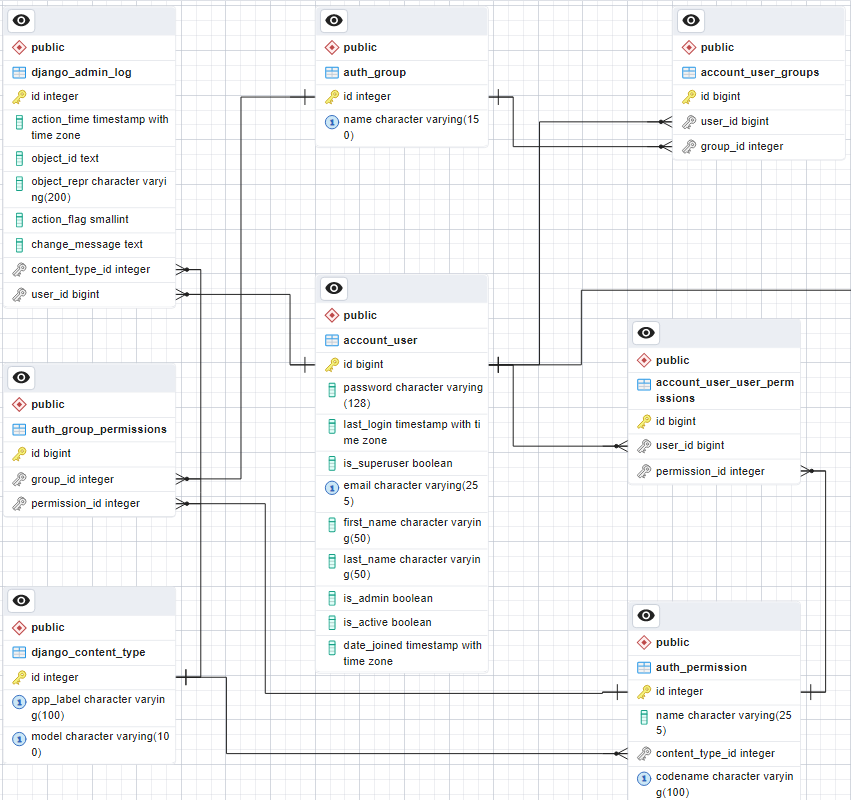
\includegraphics[scale=0.733]{inc/django}
  \caption{Данные с определенными правами, ролями и группами}
  \label{fig:fig01}
\end{figure}

Как можно заметить, на рисунке~\ref{fig:fig01} видна еще одна связь, которая уходит за пределы изображения. Это не случайно, сейчас объясним этот момент.

На рисунке~\ref{fig:fig02} показана ER-диаграмма организации структуры хранения данных для связи нашей БД с взаимодействиями на стороне back-end'а. Есть таблица, которая заполняется при первичной регистрации пользователя и служит для информации на стороне back-end'а. Кроме того, есть таблица пользователя, которая нужна только в БД и служит непосредственно для связи пользователя с медицинскими картами пациентов, которые заполняет медицинский работник при выезде.

\begin{figure}
  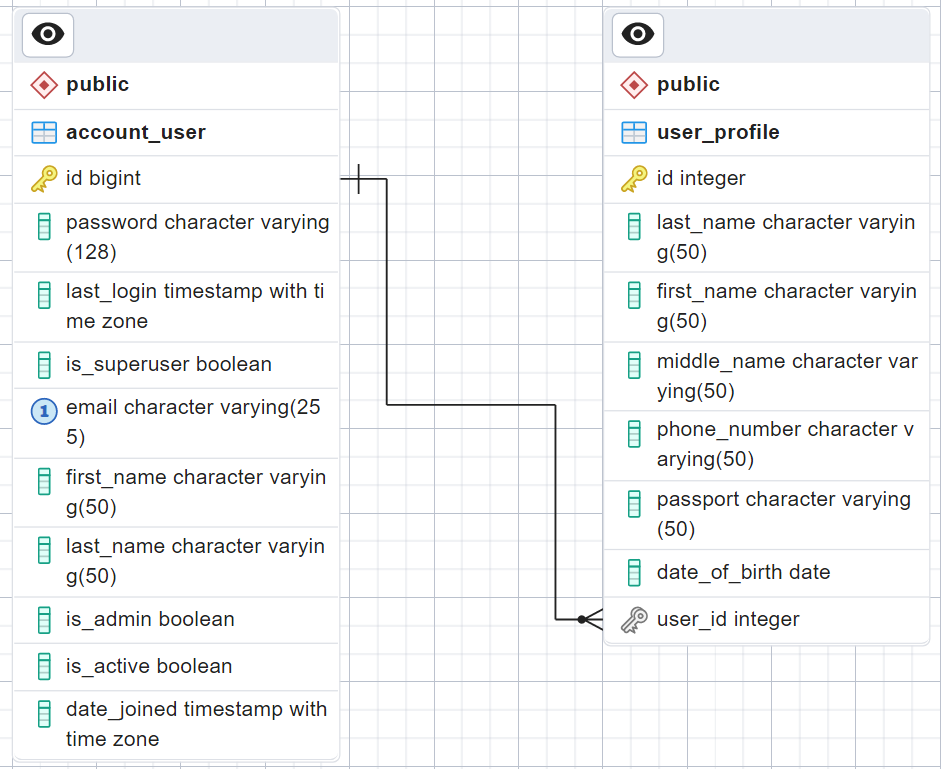
\includegraphics[scale=0.655]{inc/user_account_user_profile}
  \caption{Связи взаимодействия}
  \label{fig:fig02}
\end{figure}

На рисунке~\ref{fig:fig02} была схематично показана связь двух таблиц. Теперь приведем описание таблицы user\_profile и объясним ее назначение в нашей БД. На рисунке~\ref{fig:fig03} показана ER-диаграмма организации структуры хранения данных для пользователей нашего приложения.

\begin{figure}
  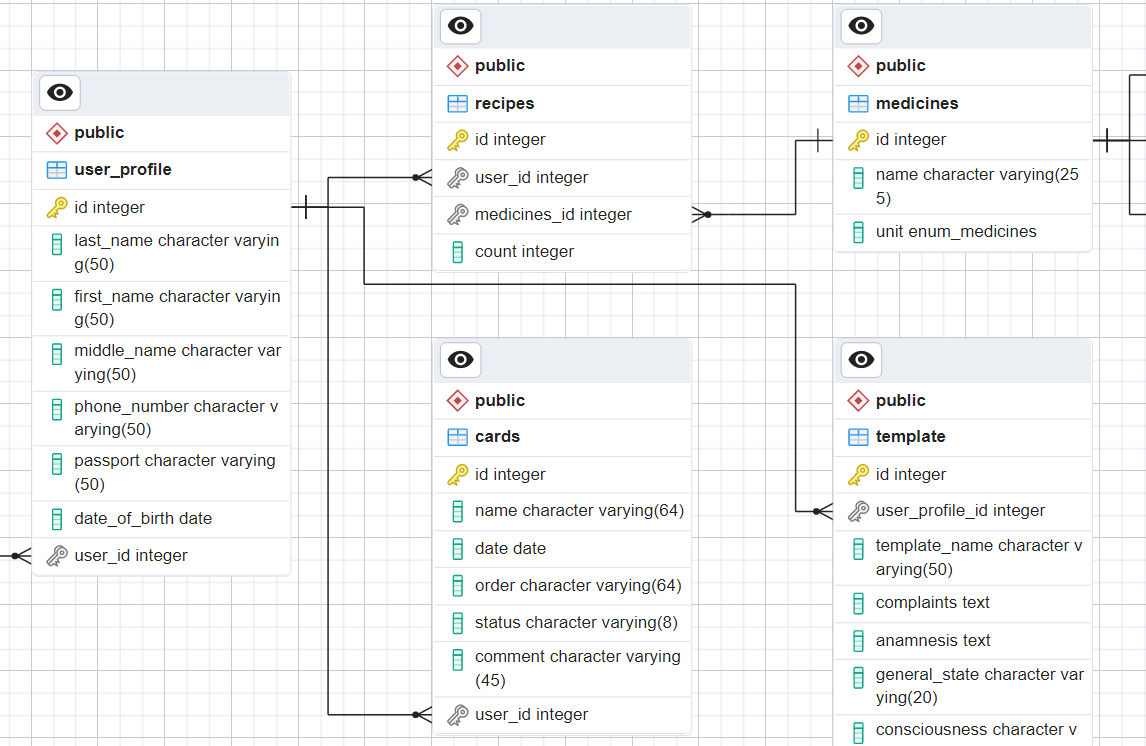
\includegraphics[scale=0.54]{inc/user_profile}
  \caption{Пользователь}
  \label{fig:fig03}
\end{figure}

Как можно заметить, в таблице medicines есть еще три связи, которые не попали на данный рисунок. Эти связи будут продемонстрированы на рисунке~\ref{fig:fig07}.

На рисунке~\ref{fig:fig04} показана ER-диаграмма организации структуры хранения данных полного взаимодействия с момента регистрации и аутентификации пользователя в приложении до связи определенного медицинского работника с шаблоном для заполнения медицинской карты при выезде к пациенту.

\begin{figure}
  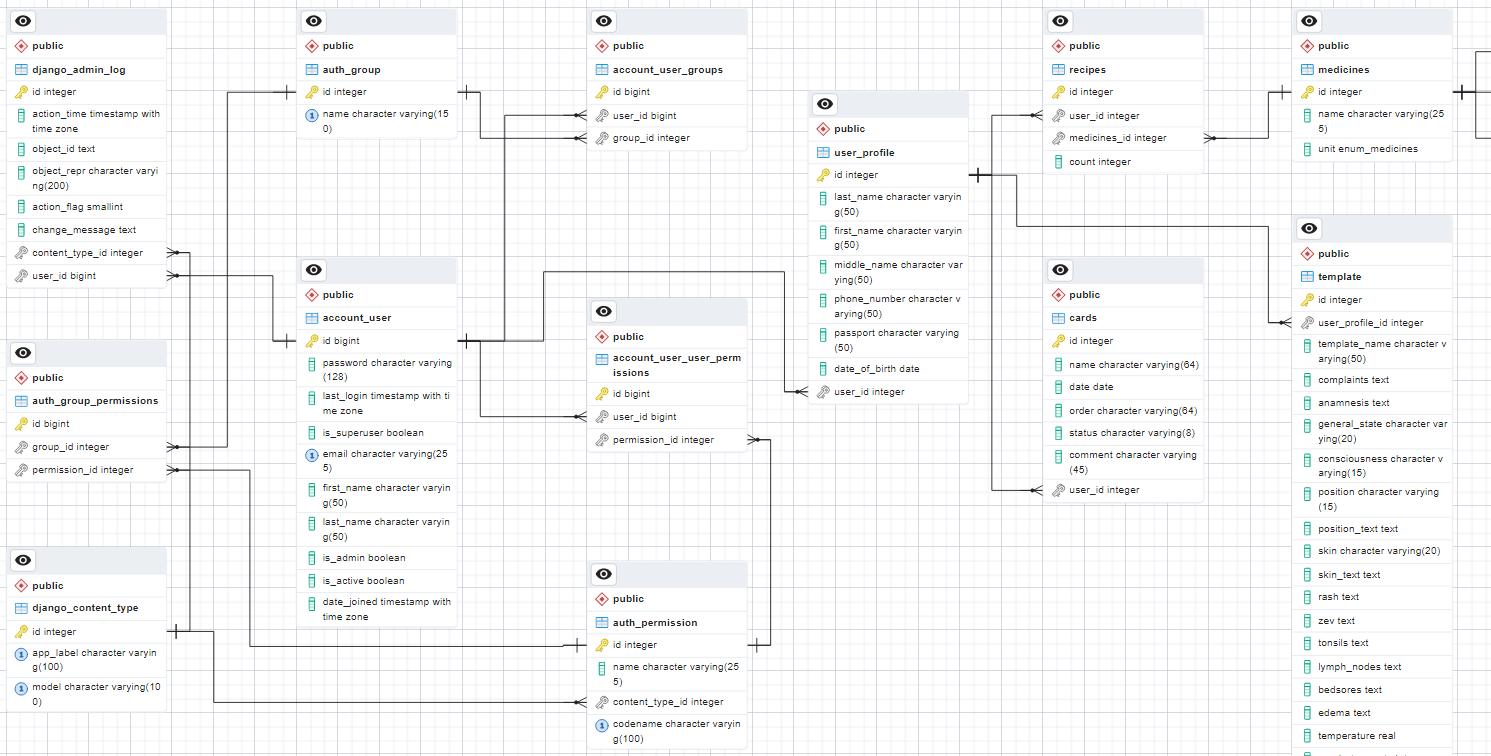
\includegraphics[scale=0.418]{inc/django_user_profile}
  \caption{Полная структура взаимодействия}
  \label{fig:fig04}
\end{figure}

На рисунке~\ref{fig:fig05} показана ER-диаграмма организации структуры хранения данных для диагнозов. Каждый диагноз относится к определённому направлению в медицине - так называемый тег. Каждый диагноз имеет свой определенный код МКБ. У диагноза есть свой определенный перечень оказания объема необходимой медицинской помощи и тактика выполнения действий. Кроме того, диагноз имеет свой так называемые формы(поддиагнозы) и относящийся уже к ним объем необходимой медицинской помощи.

\begin{figure}
  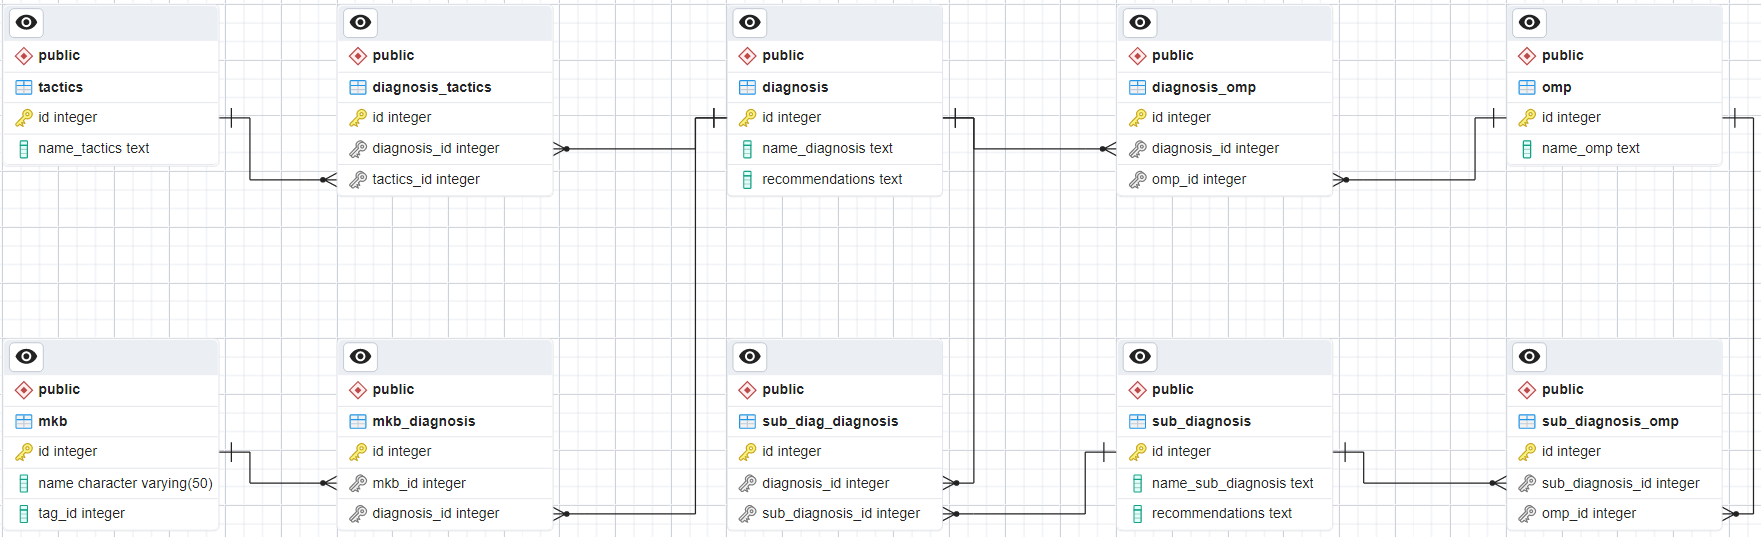
\includegraphics[scale=0.354]{inc/diagnosis}
  \caption{Диагнозы}
  \label{fig:fig05}
\end{figure}

На рисунке~\ref{fig:fig06} показана ER-диаграмма организации структуры хранения данных для заболеваний. Каждое заболевание относится к определённой категории в медицине - так называемый тег. У заболеваний есть свои определённые симптомы. Кроме того, заболевание имеет свой собственные формы и относящиеся уже к этой форме симптомы.

\begin{figure}
  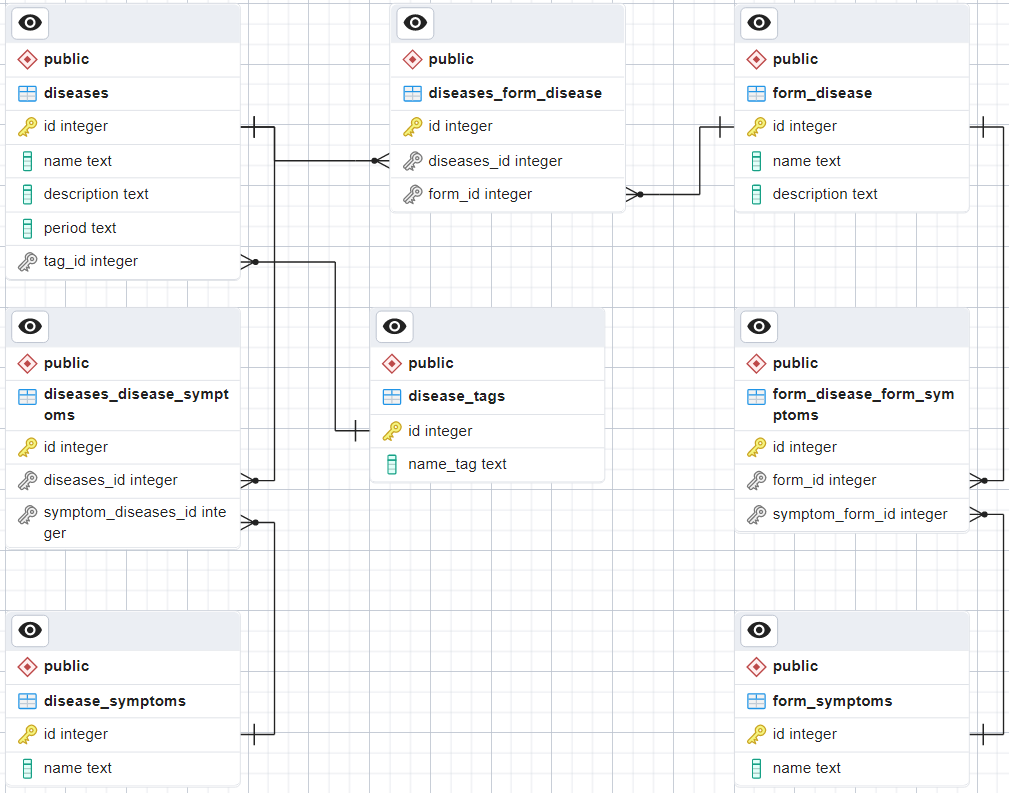
\includegraphics[scale=0.61]{inc/diseases}
  \caption{Заболевания}
  \label{fig:fig06}
\end{figure}

На рисунке~\ref{fig:fig07} показана ER-диаграмма организации структуры хранения данных для медикаментов. Каждый препарат имеет определенные противопоказания, взрослую и детскую дозировки, которые, в свою очередь зависят от конкретного диагноза.

\begin{figure}
  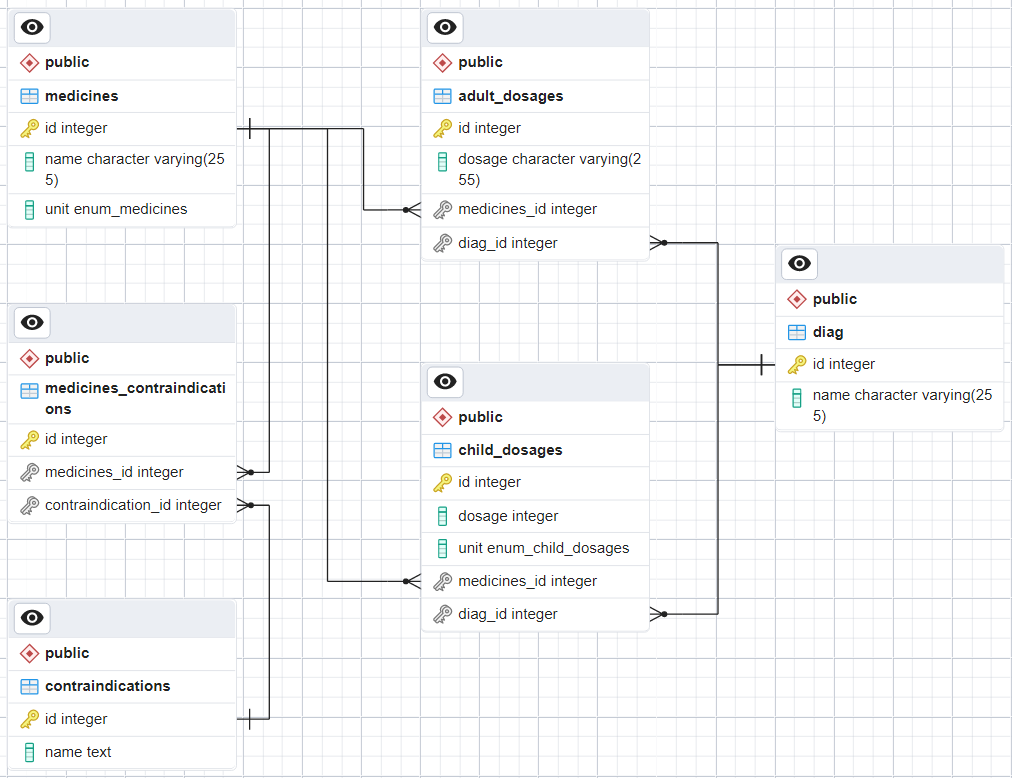
\includegraphics[scale=0.615]{inc/medicines}
  \caption{Медикаменты}
  \label{fig:fig07}
\end{figure}

Конечно, это не все таблицы, требуемые для функционала целого приложения. Медицинскому работнику иногда требуется какая-то незначительная вспомогательная информация и какой-то сложной организационной структуры эти таблицы не требуют. Вывод этих таблиц можно будет увидеть при выполнении запросов.

Таким образом, были объявлены основные таблицы БД, были рассмотрены столбцы, а именно проанализированы типы данных, а также определены ограничения для внесения конкретных значений. Этого достаточно, чтобы между таблицами сохранялась целостность данных, а вставка значений была корректной \cite{online1, online2, online3}.

Важно понимать, что перед внедрением базы данных необходимо провести тестирование и проверку ее функциональности, производительности и безопасности. Это поможет выявить потенциальные проблемы и ошибки, которые могут повлиять на работу системы. Регулярное тестирование после внедрения также является важной частью обслуживания базы данных.



\bigbreak
\textbf{Выводы по разделу}
\bigbreak

В этом разделе разбирались теоретические сведения, связанные с созданием БД. С помощью анализа организации и метода моделирования мы смогли решить задачи, связанные с определением предметной области ОНПМ и разработкой логических и физических моделей БД. На основе этих моделей были созданы таблицы в PostgreSQL, а для графического представления использовалось такое ПО как pgAdmin. Также была выполнена практическая задача, связанная с формированием системного каталога структуры БД.

Важно отметить, что разработка базы данных не является заключительным шагом. Необходимо предусмотреть систему поддержки и обслуживания, которая будет обеспечивать регулярные обновления базы данных, исправление ошибок, мониторинг производительности и резервное копирование данных. Регулярное техническое обслуживание поможет сохранить работоспособность и безопасность базы данных на протяжении всего ее существования \cite{online13}.
    \section{ЗАЩИТА БАЗЫ ДАННЫХ ОТ НЕСАНКЦИОНИРОВАННОГО ДОСТУПА}

\subsection{Основные угрозы и уязвимости}

Основные угрозы, связанные с безопасностью веб-приложений, включают:

\begin{itemize}
    \item атаки на клиентов;
    \item утечка важных данных;
    \item НСД к приложению;
    \item НСД к функциональности или контенту;
    \item раскрытие конфигурационной информации;
    \item отказ в обслуживании;
    \item атаки на ресурсы;
    \item выполнение команд ОС на сервере.
\end{itemize}

На рисунке~\ref{fig:fig08} представлена доля угроз в процентном соотношении:

\begin{figure}
  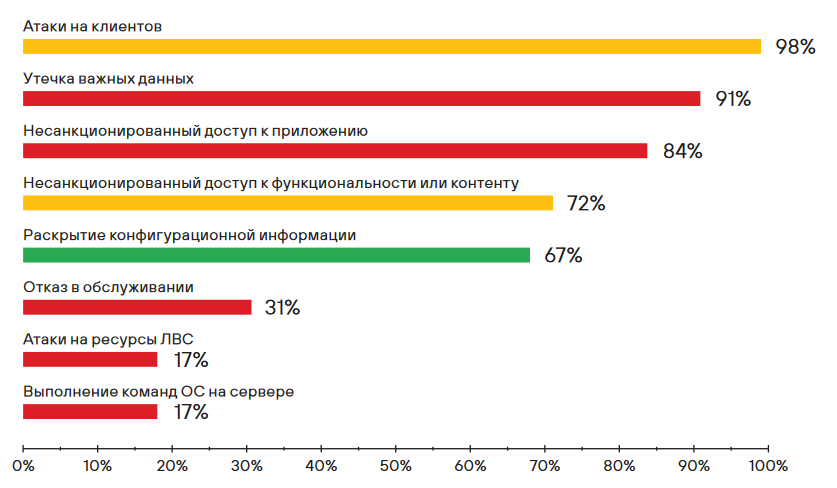
\includegraphics[scale=0.745]{inc/threats}
  \caption{Распространённые угрозы веб-приложений}
  \label{fig:fig08}
\end{figure}

Как можно заметить, утечка важных данных занимает второе место среди распространенных угроз на веб-приложения. Именно поэтому важно продумать систему защиты и хранения данных в БД.

Начиная с 2017 года актуальность атак на клиента возросла и возглавляет топ актуальных угроз. Атака вида – XSS (cross-site scripting) является каждой второй в списке атак. Сутью XSS уязвимости является возможность внедрения в веб-систему вредоносного кода и дальнейшего взаимодействия этого кода с серверами злоумышленника. Частным примером является SQL-инъекции.

SQL уязвимость основана на внедрении в запрос части произвольного SQL кода. Существует несколько способов применения SQL-инъекций использование числового входящего параметра и использование строкового входящего параметра.

Для предотвращения SQL-injection необходимо проводить правильную обработку пользовательского ввода, используя специальные методы для экранирования специальных символов и проверки вводимых данных. Например, можно использовать подготовленные запросы, которые разделяют SQL-код и данные, передаваемые в запросе, тем самым защищая приложение от выполнения злонамеренного кода.

Также важно следить за обновлением и патчингом используемых баз данных и их драйверов, чтобы избежать известных уязвимостей, которые могут быть использованы злоумышленниками для SQL-injection.

В целом, защита от SQL-инъекций требует аккуратности и внимательности в проектировании и разработке веб-приложений, а также постоянного мониторинга на наличие уязвимостей и проведения регулярных тестов на проникновение.




\subsection{Конфиденциальность персональных данных}

При разработке базы данных важно учитывать требования безопасности и конфиденциальности медицинской информации. Для этого могут быть приняты следующие меры:

\begin{itemize}
    \item шифрование данных: чувствительная медицинская информация, такая как персональные данные пациентов и медицинская история, должна быть зашифрована при хранении и передаче. Использование сильных шифровальных алгоритмов поможет защитить данные от несанкционированного доступа \cite{online11};
    \item многофакторная аутентификация: для обеспечения безопасности доступа к базе данных, особенно для медицинского персонала, следует реализовать многофакторную аутентификацию. Это требует предоставления нескольких форм идентификации, таких как пароль, биометрические данные или специальные токены, для подтверждения легитимности пользователя;
    \item управление доступом: реализация гибкой системы управления доступом поможет ограничить доступ к конфиденциальной информации только уполномоченному персоналу. Ролевая модель доступа может быть использована для определения прав доступа на основе ролей и ответственностей сотрудников;
    \item аудит и мониторинг: важно вести аудит и мониторинг доступа к базе данных для обнаружения и предотвращения несанкционированного доступа или неправомерной активности. Журналы доступа и системы мониторинга позволят выявить подозрительную активность и принять соответствующие меры;
    \item соответствие нормам и законодательству: разработка базы данных должна соответствовать применимым нормам и законодательству в области защиты персональных данных. Это включает в себя соблюдение правил по сбору, хранению, использованию и передаче медицинской информации;
    \item восстановление после катастрофы и резервное копирование: необходимо реализовать надежный план восстановления после катастрофы и резервного копирования, чтобы обеспечить доступность и целостность медицинской базы данных. Регулярные резервные копии должны выполняться, чтобы защитить от потери данных в случае сбоев системы, стихийных бедствий или кибератак. Также важно периодически тестировать процесс восстановления, чтобы убедиться в возможности точного и эффективного восстановления данных.
\end{itemize}

Анализируя вышеперечисленные пункты, можно сделать вывод, что обеспечение конфиденциальности хранения персональных данных является одним из ключевых вопросов, связанных с использованием цифровых медицинских карт и баз данных \cite{online6}.

Для обеспечения конфиденциальности данных необходимо проводить работу по защите информации и соблюдению законодательных требований. Организация должна предпринимать меры для защиты персональных данных пациентов, такие как использование паролей и шифрования данных. Кроме того, необходимо обучать медицинских работников основам информационной безопасности и контролировать доступ к информации.

Конфиденциальность хранения персональных данных пациентов - это важный аспект использования цифровых медицинских карт и организации должны принимать соответствующие меры для обеспечения безопасности информации и соблюдения законодательных требований.

PostgreSQL поддерживает множество функций для обеспечения безопасности данных, включая конфиденциальность хранения персональных данных.

Одним из ключевых механизмов для обеспечения конфиденциальности данных в PostgreSQL является использование различных методов шифрования, включая шифрование данных в пути и в покое, а также использование SSL для защиты соединений.

PostgreSQL также обеспечивает механизмы авторизации и аутентификации, которые позволяют контролировать доступ к базе данных и ее объектам, таким как таблицы и представления. Например, администраторы могут назначать различные роли и права доступа к объектам базы данных, что позволяет управлять доступом к конфиденциальным данным.

PostgreSQL также поддерживает аудиторскую функциональность, которая позволяет записывать действия пользователей в базе данных, такие как входы и выходы из системы, выполнение запросов и изменение данных. Это позволяет отслеживать и анализировать действия пользователей, чтобы обеспечить безопасность данных и защитить их от несанкционированного доступа.

В целом, PostgreSQL - это надежная и безопасная реляционная база данных, которая обеспечивает множество механизмов для защиты конфиденциальности данных, включая персональные данные пациентов.




\subsection{Использование имен пользователей, ролей и разрешений}

PostgreSQL обладает базовым механизмом защиты, включающим в себя идентификацию, аутентификацию и авторизацию. Идентификация – проверка на то, существует ли данный субъект, желающий воспользоваться данным ресурсом. Следующим шагом после идентификации следует аутентификация – проверка подлинности субъекта, в основном для этого используется паролевый метод. Конечным шагом является авторизация – предоставление необходимых прав субъекту или отказ в доступе к нужным ресурсам. Для реализации описанного механизма применяются учетные записи пользователей.

На рисунке~\ref{fig:fig09} представлено создание учетных записей для работников скорой медицинской помощи, а именно:

\begin{itemize}
    \item главный врач бригады - head\_physician;
    \item врач - doctor;
    \item фельдшер - paramedic;
    \item медсестра - nurse.
\end{itemize}

\begin{figure}
  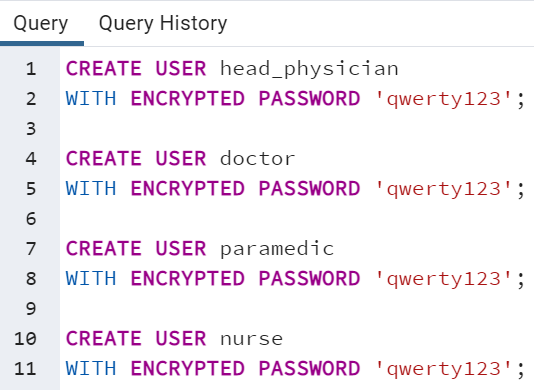
\includegraphics[scale=0.8]{inc/usernames}
  \caption{Создание учетных имен пользователей}
  \label{fig:fig09}
\end{figure}

Стоит остановиться на параметрах «CHECK\_EXPIRATION» и «CHECK\_POLICY», которые относятся к управлению паролями и их проверке при создании или изменении пользовательских данных. «CHECK\_EXPIRATION» отвечает за то, есть ли у пароля срок истечения, а «CHECK\_POLICY» определяет, должна ли использоваться паролевая политика. По умолчанию, проверка срока действия пароля и политики паролей включена в PostgreSQL, поэтому опции CHECK\_EXPIRATION и CHECK\_POLICY не нужно указывать.

Теперь нам нужно убедиться, что учетные имена пользователей и правда были созданы. Это продемонстрировано на рисунке~\ref{fig:fig10}.

\begin{figure}
  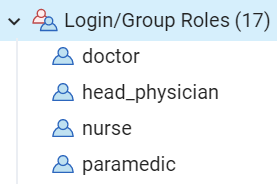
\includegraphics[scale=1]{inc/check_usernames}
  \caption{Проверка создания учетных имен пользователей}
  \label{fig:fig10}
\end{figure}

Определив учетные записи пользователей, остается лишь предоставить им необходимые разрешения, позволяющие взаимодействовать с БД. Можно отдельно каждому пользователю прописывать разрешения, но в данном случае это нецелесообразно – потому что фельдшера и медсестры должны быть одинаковые права, а у главврача и врача они такие же, только к тем правам добавляются еще другие. Выходом из этой ситуации являются роли. Роль – это объект БД, позволяющий объединять пользователей в единую группу с целью эффективного администрирования. Создание ролей и присоединение пользователей в роли продемонстрировано на рисунке~\ref{fig:fig11}.

\begin{figure}
  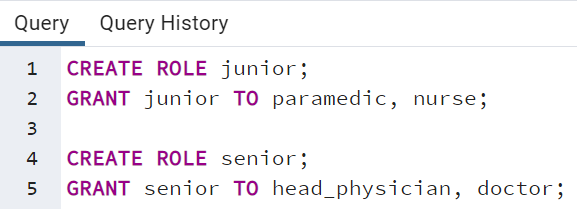
\includegraphics[scale=1]{inc/roles}
  \caption{Создание ролей и присоединение пользователей в роли}
  \label{fig:fig11}
\end{figure}

Проверим, находятся ли учетные записи в определенных ролях. Факт такого наличия изображен на рисунке~\ref{fig:fig12}.

\begin{figure}
  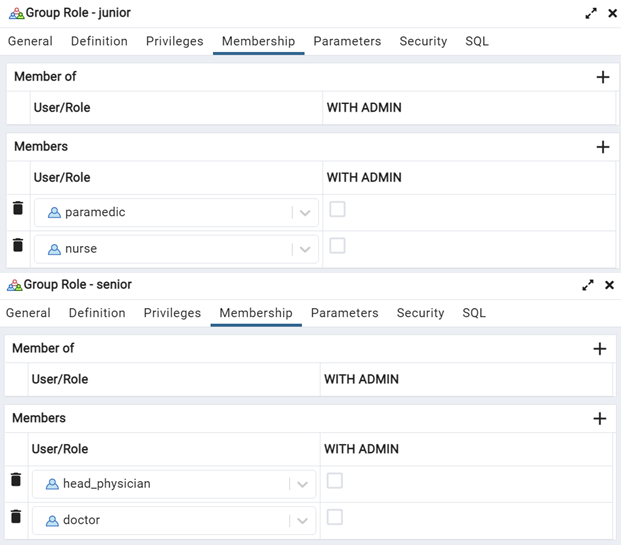
\includegraphics[scale=1.5]{inc/check_roles}
  \caption{Проверка на наличие пользователей в ролях}
  \label{fig:fig12}
\end{figure}

Создав роли для пользователей, нужно определить некоторые права, позволяющие манипулировать БД. Для этого в PostgreSQL предусмотрена возможность выдачи прав как отдельным пользователям, так и ролям.

Обозначим права, которые должны иметь роли. Роль «junior» должна иметь право на выборку всех таблиц существующей БД. Роль «senior» должна иметь право на выборку всех таблиц существующей БД, а также право на вставку, изменение и удаление значений всех таблиц, которые связаны с оказанием медицинской помощи и заполнением медкарты. На рисунке~\ref{fig:fig13} представлено присвоение ролям необходимых прав.

\begin{figure}
  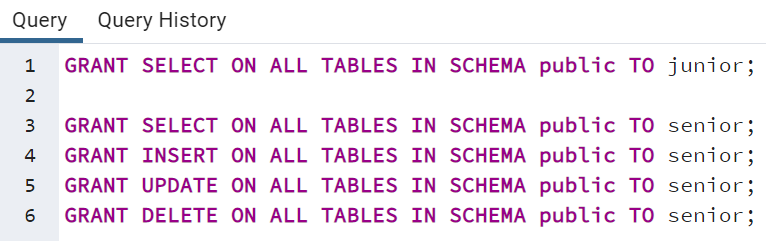
\includegraphics[scale=0.8]{inc/rights}
  \caption{Назначение прав ролям и пользователям}
  \label{fig:fig13}
\end{figure}

Стоит отметить еще одну возможность PostgreSQL. Для запрета на определенное право используется конструкция: «REVOKE action\_name ON object\_name FROM user\_name/role\_name;», при запрете права также может использоваться «CASCADE», это свойство наоборот запрещает некоторые права тем субъектам, которым оно выдавалось. Помимо выдачи и запрета прав есть третья возможность – отмена прав, она имеет следующий синтаксис: «REVOKE action\_name ON object\_name FROM user\_name/role\_name [CASCADE];», свойство «CASCADE» используется для отмены прав у тех субъектов, которым данный пользователь выдал. Стоит обратить внимание, что для использования команды REVOKE в PostgreSQL необходимо иметь соответствующие привилегии администратора базы данных.

pgAdmin также позволяет просмотреть права ролей у каждой таблицы. На рисунке~\ref{fig:fig14} изображены предоставленные права к таблице «Медикаменты».

\begin{figure}
  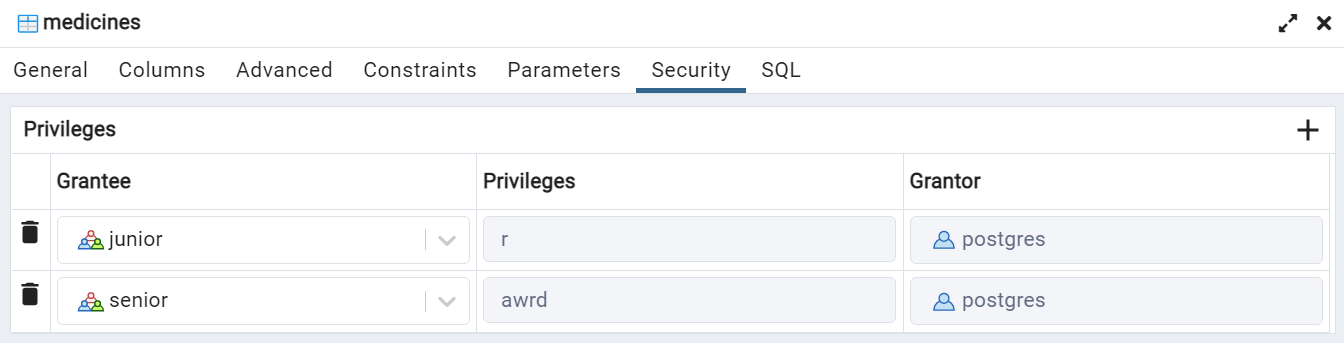
\includegraphics[scale=0.46]{inc/rights_tables}
  \caption{Проверка ролей на их возможные права в таблице}
  \label{fig:fig14}
\end{figure}





\subsection{Шифрование базы данных}

Вторым базовым механизмом защиты, реализующимся в PostgreSQL, от НСД является шифрование БД. Шифрование – это преобразование исходной информацию в данные, которые теряют иной смысл, не зная секретного слова или алгоритма, преобразовывающие данные обратно в смысловую информацию.

Самый популярный способ зашифровать информацию, хранящуюся в БД – это прозрачное шифрование данных. Преимущество такого вида шифрования заключается в том, что конечные пользователи могут даже и не знать, что применяется защита информации.

Прозрачное шифрование, также известное как шифрование в режиме реального времени, представляет собой способ защиты данных, при котором шифрование и расшифровка осуществляются автоматически без участия пользователя. Этот метод основан на работе специального драйвера, который функционирует в фоновом режиме и следит за всеми операциями с данными. Его главная цель заключается в предотвращении атак, направленных на получение данных путем обхода операционной системы, например, через загрузку из другой ОС или использование альтернативных методов.

Перед тем, как перейти к шифрованию, следует, на всякий случай, сделать резервную копию БД. Для этого следует включить pgAgen.

Затем выбираем нужную БД, вызываем контекстное меню, в нем выбираем опцию «создать резервную копию».

Создав резервную копию БД, можно приступать к процессу шифрования. Этот процесс происходит в несколько этапов:

\begin{itemize}
    \item создание главного ключа БД;
    \item создание сертификата;
    \item создание ключа шифрования;
    \item запуск процесса шифрования;
    \item проверка состояния шифрования.
\end{itemize}

Главный ключ БД – это ключ, который применяется для шифрования других ключей, использующихся для реализации шифрования в БД. Для его создания применяется следующая конструкция: «CREATE MASTER KEY ENCRYPTION BY PASSWORD 'password';».

Следующим шагом будет создание сертификата. Сертификат – это объект безопасности, имеющий подпись. Этот объект хранит в себе ключи шифрования. Для создания данного объекта применяется следующая конструкция: «CREATE CERTIFICATE name\_db\_and\_cert WITH SUBJECT 'description';».

Последним подготовительным этапом перед началом шифрования БД является создание ключа шифрования. Именно этим ключом будет происходить шифрование БД, а сам ключ будет находиться в сертификате, созданном заранее. Для его создания требуется применять следующий шаблон: «CREATE DATABASE ENCRYPTION KEY WITH ALGORITHM = AES\_128 ENCRYPTION BY SERVER CERTIFICATE cert\_name;».

Следующий шаг является необязательным, но его желательно выполнять. При создании главного ключа, сертификата и ключа шифрования рекомендуется создание резервных копий этих объектов безопасности. Для создания резервной копии ключа шифрования можно использовать команду pg\_dump, которая создаст резервную копию всей базы данных, включая ключи шифрования: «pg\_dump dbname > backup\_file\_name;».

Все объекты безопасности проинициализированы, также для критических объектов были созданы резервные копии. Теперь можно приступать к шифрованию БД. Для начала данного процесса используется следующий пакет команд: «UPDATE table\_name SET column\_name = pgp\_sym\_encrypt(column\_name, 'key\_password');».

Осталось лишь проверить, работает ли ключ шифрования для БД. Для этого используются системные БД «pg\_database\_encryption». Нас интересует столбец is\_encrypted, если шифрование завершилось успешно, то столбец принимает значение 1.

Но, сказать честно, нас мало интересует сквозное шифрование всей БД. Ведь сквозное шифрование всей базы данных может иметь несколько негативных аспектов:

\begin{itemize}
    \item высокая нагрузка на производительность: Шифрование и дешифрование больших объемов данных может быть ресурсоемким процессом, что может замедлить операции чтения и записи в базе данных. Это особенно актуально для приложений с высокой нагрузкой или большим количеством одновременных пользователей;
    \item ограничения по поиску и сортировке: Шифрованные данные нельзя эффективно искать или сортировать без их предварительного расшифрования. Если в базе данных необходимо выполнять сложные операции поиска или агрегации данных, то сквозное шифрование может существенно затруднить выполнение этих операций;
    \item управление ключами: Для сквозного шифрования необходимо использовать сильные шифровальные ключи, их генерацию, хранение и управление. Ключи должны быть доступны для расшифровки данных, что может представлять риск безопасности, особенно если ключи утекают или попадают в неправильные руки;
    \item затрудненная администрация: Сквозное шифрование требует дополнительного управления и конфигурации в базе данных и приложениях. Это может усложнить администрирование базы данных и требовать дополнительных усилий для поддержки и масштабирования системы;
    \item ограниченные возможности обработки данных: Шифрование данных делает их недоступными для анализа, обработки и использования в алгоритмах машинного обучения или других высокоуровневых операциях, которые требуют доступа к исходным данным.
\end{itemize}

Вместо сквозного шифрования всей базы данных может быть целесообразнее использовать частичное шифрование, где шифруются только конкретные конфиденциальные данные или поля, сохраняя остальные данные в незашифрованном виде. Это позволяет более гибко балансировать безопасность и производительность системы. Именно так мы и поступим. Будем шифровать только те данные, которые могут определенно точно идентифицировать личность человека.

Воспользуемся модулем pgcrypto для симметричного шифрования выборочных данных. Но для начала убедимся, что модуль установлен. На рисунке~\ref{fig:fig15} можно видеть, что у нас все готово к работе.

\begin{figure}
  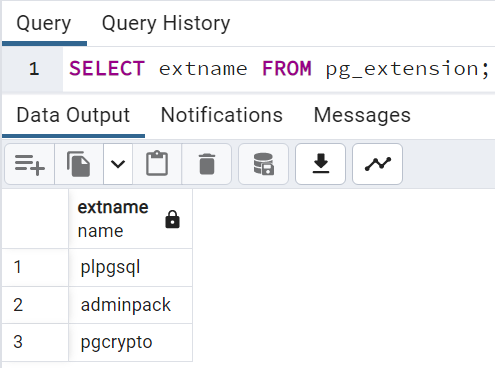
\includegraphics[scale=0.52]{inc/pgcrypto}
  \caption{Проверка наличия модуля pgcrypto}
  \label{fig:fig15}
\end{figure}

Можно шифровать и расшифровывать столбцы в таблицах в созданной БД:

\begin{itemize}
    \item для шифрования используется следующий шаблон: «UPDATE mytable SET mycolumn = pgp\_sym\_encrypt(mycolumn, 'mysecretkey');»;
    \item для расшифрования используется следующий шаблон: «SELECT pgp\_sym\_decrypt(mycolumn, 'mysecretkey') AS decrypted\_data FROM mytable;».
\end{itemize}

На рисунке~\ref{fig:fig16} приведены данные в чистом виде без шифрования.

\begin{figure}
  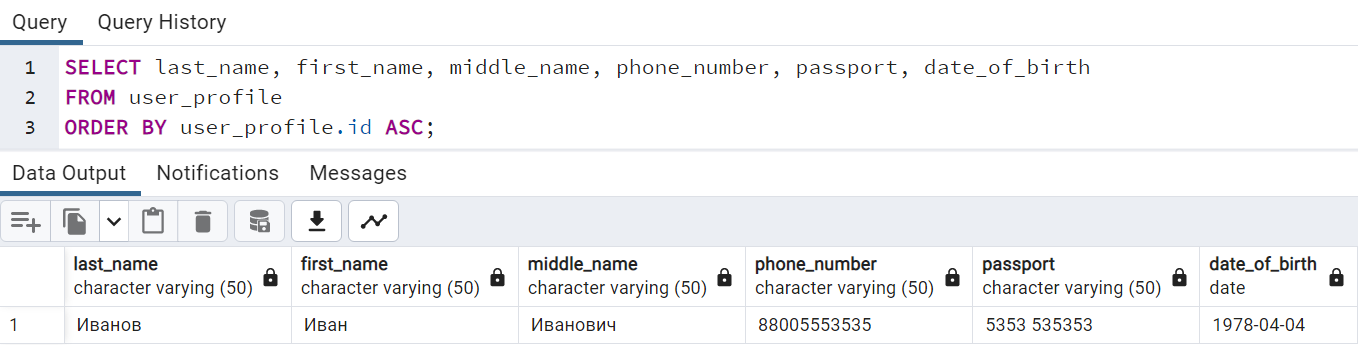
\includegraphics[scale=0.456]{inc/table_user_profile}
  \caption{Изначальные данные таблицы user\_profile}
  \label{fig:fig16}
\end{figure}

На рисунке~\ref{fig:fig17} представлен пример того, как шифруются некоторые столбцы.

\begin{figure}
  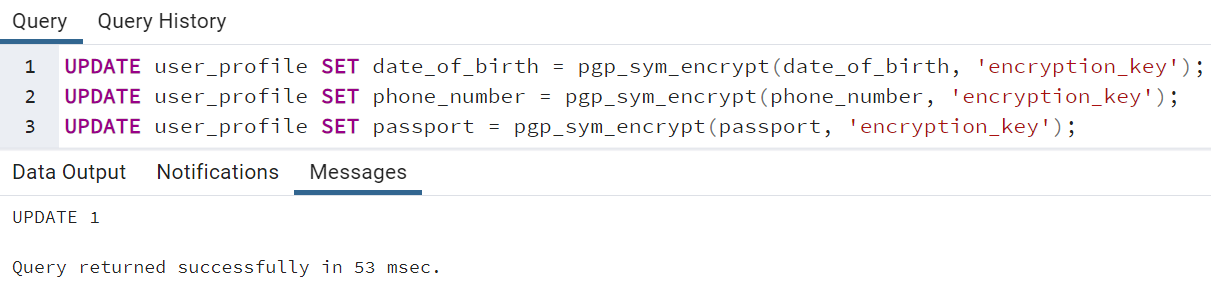
\includegraphics[scale=0.51]{inc/encryption}
  \caption{Шифрование некоторых данные таблицы user\_profile}
  \label{fig:fig17}
\end{figure}

Теперь убедимся, что наши данные и правда были зашифрованы. Это можно увидеть на рисунке~\ref{fig:fig18}.

\begin{figure}
  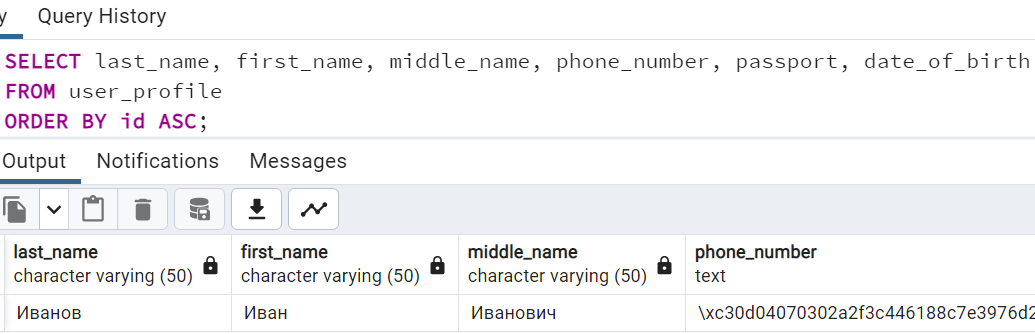
\includegraphics[scale=0.6]{inc/encrypted_table}
  \caption{Проверка шифрования некоторых данных таблицы user\_profile}
  \label{fig:fig18}
\end{figure}

На рисунке~\ref{fig:fig18} видно, что столбец с паспортными данными успешно зашифрован и можно не переживать за конфиденциальность хранения персональных данных. Но что теперь делать, нужно же не только хранить, но и получать данные из таблицы. Для этого при выполнении запроса вызывается функция расшифрования с тем самым ключом, который использовался при шифровании. На рисунке~\ref{fig:fig19} продемонстрирован запрос на получения данных в зашифрованного столбца с процессом расшифрования по ходу выполнения.

\begin{figure}
  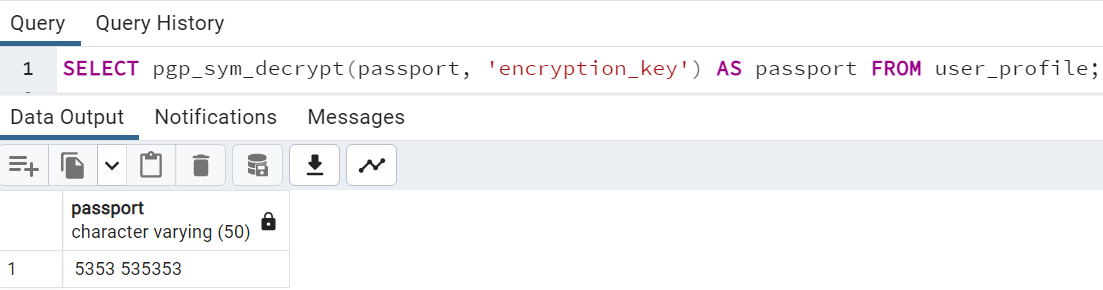
\includegraphics[scale=0.847]{inc/decryption}
  \caption{Получение данных зашифрованного столбца с расшифрованием в процессе выполнения запроса}
  \label{fig:fig19}
\end{figure}

В конечном итоге, после расшифрования всех данных, мы получим идентичные данные, что были до процесса шифрования. На рисунке~\ref{fig:fig20} можно увидеть, что целостность данных не была нарушена после процессов шифрования и дешифрования данных.

\begin{figure}
  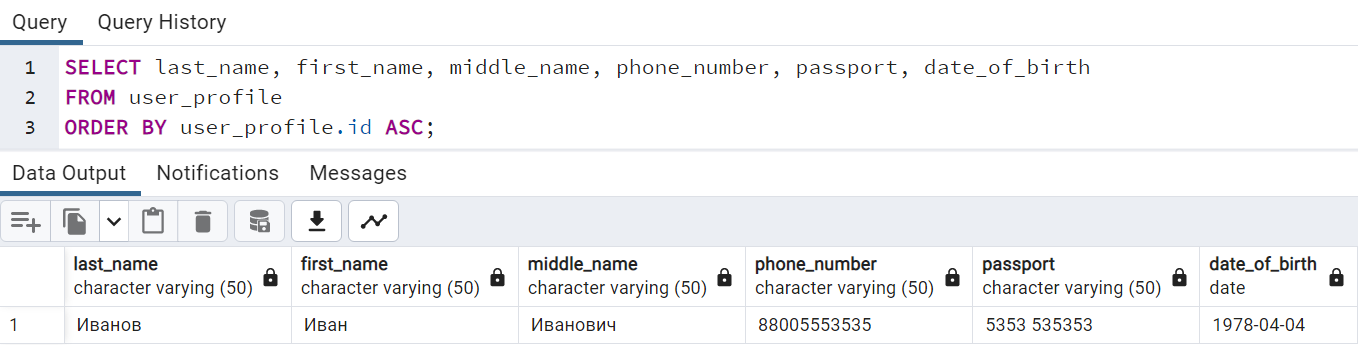
\includegraphics[scale=0.456]{inc/table_user_profile}
  \caption{Подтверждение целостности данных}
  \label{fig:fig20}
\end{figure}



\subsection{Порты}

Порт – это некоторое идентифицирующее число от 1 до 65535, позволяющее протоколам взаимодействовать друг с другом на транспортном уровне модели OSI.

На самом деле, у PostgreSQL сервера по умолчанию установлен только один порт, и это TCP порт.

PostgreSQL использует TCP/IP для обмена данными между клиентами и сервером. По умолчанию, порт TCP для PostgreSQL установлен на 5432. TCP 5432: database engine, используется для подключения к СУБД. Этот порт можно изменить при настройке сервера \cite{online7}.

Несмотря на то, что UDP не используется для коммуникации между клиентами и сервером PostgreSQL, есть несколько расширений, таких как pgpool-II, которые могут использовать UDP для взаимодействия между серверами PostgreSQL.

Таким образом, можно сказать, что PostgreSQL сервер по умолчанию использует только один порт TCP для обмена данными между клиентами и сервером.

Хорошей практикой является смена портов на другие, чтобы при случае атаки порты пришлось перебирать методом грубого подбора, а не использовать установленные по умолчанию. По данным IANA, порты 834-846 являются свободными, поэтому мы их можем использовать.

Для изменения порта, используемого PostgreSQL, можно внести изменения в конфигурационный файл postgresql.conf, который находится в каталоге данных PostgreSQL.

В файле postgresql.conf необходимо изменить параметр port на желаемое значение порта. Например, если вы хотите использовать порт 840 вместо стандартного порта 5432, необходимо изменить строку: port = 5432 на port = 840. После этого нужно перезапустить PostgreSQL, чтобы изменения вступили в силу.

Также можно использовать параметр командной строки -p при запуске сервера PostgreSQL для указания порта. Например, чтобы запустить PostgreSQL на порту 840, необходимо использовать команду: postgres -p 840, но в этом случае необходимо убедиться, что порт 840 свободен и не используется другим приложением на сервере.

Помимо смены порта, слушающий входящие соединения, можно отключить PostgreSQL Server. PostgreSQL Server – это одна из служб PostgreSQL, отвечающая за прослушивание запросов. Если эту службу отменить, то для установления соединения придется явно указывать номер порта, что обеспечивает дополнительную безопасность. Для остановки этой службы требуется просто ввести sudo systemctl stop postgresql в командной строке.



\subsection{Брандмауэр}

Брандмауэр – это программный межсетевой экран, имеющийся в ОС Windows. В свою очередь межсетевой экран – это элемент локальной сети, осуществляющий мониторинг активности в данной сети, а именно фильтрацию сетевого трафика по заранее описанным правилам. PostgreSQL Server функционирует на ОС Windows, поэтому рекомендуется использовать Брандмауэр вместе с программно-аппаратным межсетевым экраном. Такое сочетание позволяет повысить уровень защищенности за счёт использования дополнительных механизмов защиты информации. Также Брандмауэр обеспечивает не только защищенность от НСД, но и от поступающего вредоносного трафика в принципе.

Как было описано выше, межсетевой экран анализирует сетевой трафик и отклоняет его, если он считается подозрительным. Выше мы поменяли стандартный TCP/UDP порт 5432 на 840, теперь нужно объявить правило в межсетевом экране, что публичная сеть не может ссылаться на этот порт. Для этого заходим в Монитор Брандмауэра Защитника Windows в режиме повышенной безопасности и создадим новое правило. Далее определяем, что правило создается для порта, затем вписываем наш нужный порт, после этого разрешаем подключение, после этого исключаем публичный доступ, и в конце сохраняем наше правило.


\bigbreak
\textbf{Выводы по разделу}
\bigbreak

В этом разделе разбирались аспекты, связанные с безопасностью. Для защиты от НСД внутренними средствами PostgreSQL была реализована авторизация пользователей, а также им были назначены необходимые минимальные права для работы с БД, что позволило осуществить легитимный доступ к информации. Для повышения конфиденциальности информации использовалось шифрование информации на уровне столбцов при помощи библиотеки pgcrypto. Кроме того, при помощи шифрования файлы БД были защищены от кражи на физических носителях. А изменение портов и использование Брандмауэра позволило защититься на сетевом уровне. В совокупности была выполнена задача определения защитных мер БД.
    \section{ТЕСТИРОВАНИЕ И ОПТИМИЗАЦИЯ ПРОИЗВОДИТЕЛЬНОСТИ}

\subsection{Методы и инструменты тестирования}

Перед заключительным этапом проводят тестирование базы данных и ее оптимизацию. На этом этапе производятся проверки корректной и эффективной работы базы данных. Кроме того, выполняются тесты производительности, определяются проблемы с ней и соответственно решение этих проблемы путем оптимизации запросов, индексов и настройки СУБД PostgreSQL.

Для тестирования базы данных можно использовать различные методы и инструменты, такие как:

Существуют различные методы и инструменты для проверки базы данных, включая:

\begin{itemize}
    \item модульное тестирование: это проверка отдельных компонентов базы данных, таких как хранимые процедуры, триггеры, функции и другие;
    \item интеграционное тестирование: это проверка совместной работы базы данных с приложением, которое использует эту базу данных;
    \item нагрузочное тестирование: это проверка производительности базы данных в условиях высокой нагрузки;
    \item тестирование безопасности: это проверка уязвимостей базы данных и соответствия ее требованиям безопасности;
    \item ручное тестирование: это проверка базы данных на соответствие требованиям и наличие ошибок, которую выполняет тестировщик вручную.
\end{itemize}



\subsection{Нагрузочное тестирование и оптимизация производительности}

Нагрузочное тестирование БД в PostgreSQL - это процесс измерения производительности и стабильности базы данных при большой нагрузке. Это необходимо для определения максимального количества пользователей и запросов, которые могут быть обработаны базой данных, без ухудшения ее производительности.

Для проведения нагрузочного тестирования БД в PostgreSQL, необходимо выполнить следующие шаги:

\begin{itemize}
    \item определить сценарии использования БД: определить типы запросов, которые будут отправлены к БД, и количество пользователей, которые будут использовать приложение одновременно;
    \item подготовить тестовые данные: создать тестовые данные, которые будут использоваться при выполнении запросов в тестовом окружении. Важно создать реалистичные тестовые данные, чтобы результаты нагрузочного тестирования были максимально близки к реальной нагрузке;
    \item настроить окружение для нагрузочного тестирования: убедиться, что база данных и приложение настроены правильно, чтобы обеспечить максимальную производительность и стабильность;
    \item запустить нагрузочное тестирование: выполнить тестовые сценарии использования БД в тестовом окружении и измерить производительность базы данных, используя метрики, такие как скорость ответа, время выполнения запросов, количество ошибок и использование ресурсов;
    \item анализ результатов: проанализировать результаты нагрузочного тестирования, чтобы определить максимальную нагрузку, которую может выдержать база данных, и определить узкие места, которые могут быть оптимизированы.
\end{itemize}

При тестировании в PostgreSQL можно использовать специальные инструменты, такие как pgbench и Apache JMeter, чтобы автоматизировать процесс выполнения тестовых сценариев и сбора метрик производительности. Важно понимать, что результаты нагрузочного тестирования могут изменяться в зависимости от настроек и конфигурации сервера и базы данных, поэтому рекомендуется проводить тестирование на реальном оборудовании, которое будет использоваться в итоговой среде.

\begin{itemize}
    \item pgbench: это инструмент, входящий в стандартный комплект поставки PostgreSQL. Он предназначен для проведения нагрузочного тестирования на уровне SQL-запросов \cite{online10};
    \item pgBadger: это инструмент для анализа логов PostgreSQL. Он позволяет анализировать логи запросов и генерировать отчеты о производительности базы данных;
    \item HammerDB: это инструмент для тестирования производительности баз данных. Он поддерживает PostgreSQL и позволяет тестировать производительность базы данных на различных уровнях нагрузки;
    \item Sysbench: это инструмент, который может быть использован для тестирования производительности базы данных PostgreSQL. Он позволяет тестировать производительность базы данных на уровне SQL-запросов и многопоточности.
\end{itemize}

Важно помнить, что результаты нагрузочного тестирования БД PostgreSQL могут зависеть от конкретной конфигурации сервера и структуры данных, а также от условий использования базы данных в реальном мире. Поэтому результаты тестирования должны быть интерпретированы с осторожностью и использованы для оптимизации конкретной базы данных.

Оптимизация производительности базы данных PostgreSQL может включать в себя ряд мероприятий, чтобы ускорить выполнение SQL запросов и обеспечить более эффективную работу БД. Вот основные подходы, которые можно эффективно использовать для оптимизации БД PostgreSQL \cite{online8, online9}:

\begin{itemize}
    \item создание правильных индексов: индексы ускоряют выполнение запросов, позволяя PostgreSQL быстро находить нужные данные. Убедитесь, что у вас есть индексы на часто используемые столбцы в запросах, а также на столбцы, используемые в условиях WHERE и JOIN и фильтрации данных, может значительно ускорить выполнение запросов;
    \item оптимизация запросов: оптимизация запросов, такая как использование подзапросов, объединения и группировки данных, может улучшить производительность запросов и уменьшить количество запросов, необходимых для выполнения операции;
    \item разделение данных на отдельные таблицы: если у нас есть большие таблицы, то не следует хранить большие объемы данных в одной таблице. Разделение этих данных на отдельные таблицы или партицирование может помочь ускорить выполнение запросов. Это позволяет более эффективно управлять объемом данных, используемых при выполнении запросов;
    \item оптимизация схемы базы данных: иногда изменение структуры базы данных может привести к улучшению производительности. Например, использование более эффективных типов данных, уменьшение количества NULL значений или устранение избыточных таблиц и связей;
    \item использование кэширования: если важна скорость выполнения, то можно использовать кэширование для часто запрашиваемых данных. Использование кэширования запросов может значительно улучшить производительность, позволяя избежать выполнения сложных запросов, возвращая результаты из кэша. Это особенно полезно для запросов, которые выполняются часто и имеют статические результаты;
    \item оптимизация запросов на запись: если есть интенсивная нагрузка на запись данных, то различные техники, такие как пакетная вставка (batch insert), использование транзакций и пакетных обновлений, могут помочь ускорить процесс записи данных;
    \item предварительная компиляция запросов: в PostgreSQL есть возможность предварительной компиляции запросов (prepared statements), что позволяет повторно использовать выполненные запросы и сократить накладные расходы на компиляцию. Предварительную компиляцию стоит использовать для запросов, которые выполняются многократно с различными параметрами;
    \item настройка конфигурации PostgreSQL: немаловажное значение имеет изучение и настройка параметров конфигурации PostgreSQL в соответствии с требованиями конкретной системы. Некоторые параметры, которые можно настроить, включают размер буферов, параллелизм выполнения запросов и максимальное количество одновременных соединений;
    \item обновление до последней версии PostgreSQL: немаловажное значение имеет актуальность поддерживаемого ПО, поэтому рекомендуется использовать последнюю стабильную версию PostgreSQL. Каждое новое обновление может содержать оптимизации и улучшения производительности, которые могут существенно повысить скорость выполнения запросов;
    \item настройка памяти и дискового пространства: правильная настройка памяти и дискового пространства может существенно повлиять на производительность PostgreSQL. Следует выделять достаточное количество памяти для работы с базой данных. Кроме того, система должна иметь достаточное дисковое пространство для хранения данных и временных файлов;
    \item использование материализованных представлений: материализованные представления - это предварительно вычисленные результаты запросов, сохраняемые в виде таблиц. Они могут быть особенно полезны, если имеются сложные запросы с большими объемами данных, которые выполняются часто. Материализованные представления позволяют значительно сократить время выполнения запросов;
    \item настройка параллелизма: PostgreSQL поддерживает параллельное выполнение запросов, что может значительно ускорить обработку больших объемов данных. Можно настроить параметры параллелизма в зависимости от характеристик системы и требований к производительности;
    \item горизонтальное масштабирование: если даже после оптимизации базы данных путем проведения вышеперечисленных манипуляций все еще возникают проблемы с производительностью , можно рассмотреть вариант горизонтального масштабирования. Распределение данных на несколько серверов может помочь справиться с высокой нагрузкой и улучшить производительность;
    \item оптимизация настройки сервера: настройка параметров сервера PostgreSQL, таких как размер буфера и количество параллельных запросов, может улучшить производительность базы данных.
\end{itemize}

Важно проводить тестирование на реалистичных тестовых данных и сценариях использования, чтобы получить наиболее точные результаты. Также при проведении нагрузочного тестирования БД PostgreSQL необходимо учитывать следующие факторы:

\begin{itemize}
    \item объем данных: чем больше объем данных в базе данных, тем больше ресурсов требуется для обработки запросов. Поэтому важно учитывать объем данных при выборе конфигурации сервера и оптимизации производительности;
    \item конфигурация сервера: настройка сервера PostgreSQL имеет большое значение для производительности базы данных. Например, увеличение размера буфера может ускорить выполнение запросов, но при этом может потребовать больше памяти;
    \item структура данных: структура таблиц и связей между ними может влиять на производительность базы данных. Например, использование ненормализованных таблиц может привести к медленной работе базы данных;
    \item распределение запросов: распределение запросов между разными серверами или узлами может увеличить производительность и снизить нагрузку на базу данных,
\end{itemize}

С учётом вышеперечисленных возможностей для оптимизации и тестирования, было проведено нагрузочное тестирование полностью готовой, оптимизированной и заполненной реальными данными БД для полноценного функционирования web-приложения onmp.ru с помощью модуля PostgreSQL - pgbench.

Для проведения нагрузочного тестирования требуется:

\begin{itemize}
    \item инициализировать базу данных с помощью pgbench. Это создаст необходимые таблицы и заполнит их тестовыми данными:

    «pgbench -i -s 100 database\_name».

    Флаг -s 100 указывает на размер масштабируемости данных, где 100 означает, что будет создано в 100 раз больше строк, чем количество таблиц. Можно изменить это значение в соответствии с потребностями в тестировании;
    \item запускаем нагрузочное тестирование с помощью pgbench. Ниже приведен пример команды, которая запускает тест с 10 параллельными клиентами и общим числом транзакций 1000:
    
    «pgbench -c 10 -j 10 -t 1000 database\_name».
    
    Флаг -c 10 указывает на количество параллельных клиентов, -j 10 указывает на количество параллельных потоков (обычно выбирают такое же значение, как и -c), а -t 1000 указывает на общее количество транзакций для выполнения;
    \item далее анализируем результаты тестирования, которые будут выведены в консоль. Они включают среднее время выполнения транзакции, количество транзакций в секунду и другие метрики производительности;
    \item затем будем просто изменять параметры команды pgbench, такие как количество клиентов, количество потоков и общее количество транзакций, чтобы провести более интенсивное или длительное тестирование.
\end{itemize}

С подробными результатами нагрузочного тестирования можно ознакомиться в приложении Б. По полученным результатам можно увидеть и смело сделать вывод, что разработанная база данных в полной мере выдерживает нагрузки при больших объемах хранимых и обрабатываемых данных. Кроме того, при одновременном подключении порядка 50-80 пользователей, система выдержала нагрузку и задержка на подключение пользователя к сессии составляет всего около 0.5 секунд, что никак отрицательно не отражается на работоспособности и корректном функционировании web-приложения.

Тестирование БД PostgreSQL является важным этапом при разработке и оптимизации базы данных. Оно позволяет выявить узкие места в работе базы данных и произвести необходимую оптимизацию, чтобы обеспечить максимальную производительность и стабильность приложения.

Стоит отметить, что после внедрения базы данных необходимо проводить анализ ее использования и результата. Это позволит выявить потенциальные улучшения и оптимизации процессов работы с медицинской информацией. На основе анализа можно внести изменения в структуру базы данных, внедрить новые функциональные возможности или улучшить существующие.



\subsection{Выполнение запросов}

После того, как мы разобрались с видами тестирования, оптимизацией памяти и скорости выполнения запросов, самое время продемонстрировать полученные результаты.

На рисунке~\ref{fig:fig21} представлен SQL запрос к таблицам медикаментов, представленных на рисунке~\ref{fig:fig07}.

\begin{figure}
  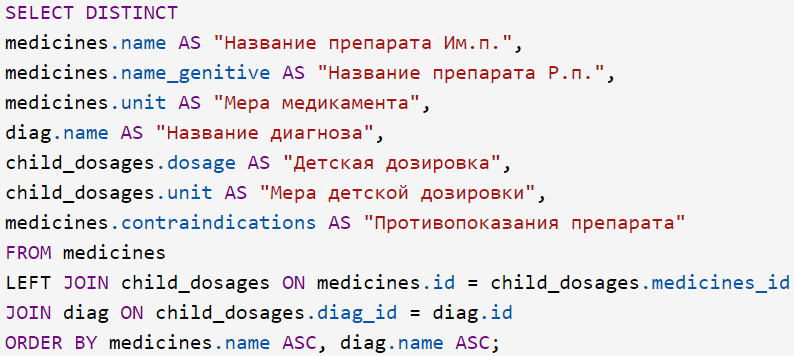
\includegraphics[scale=0.78]{inc/sh_all_ch_med}
  \caption{SQL запрос получения всех медикаментов}
  \label{fig:fig21}
\end{figure}

Запрос есть, теперь нужно посмотреть корректность выводимых данных. На рисунке~\ref{fig:fig22} представлен вывод SQL запроса с рисунка~\ref{fig:fig21}.

\begin{figure}
  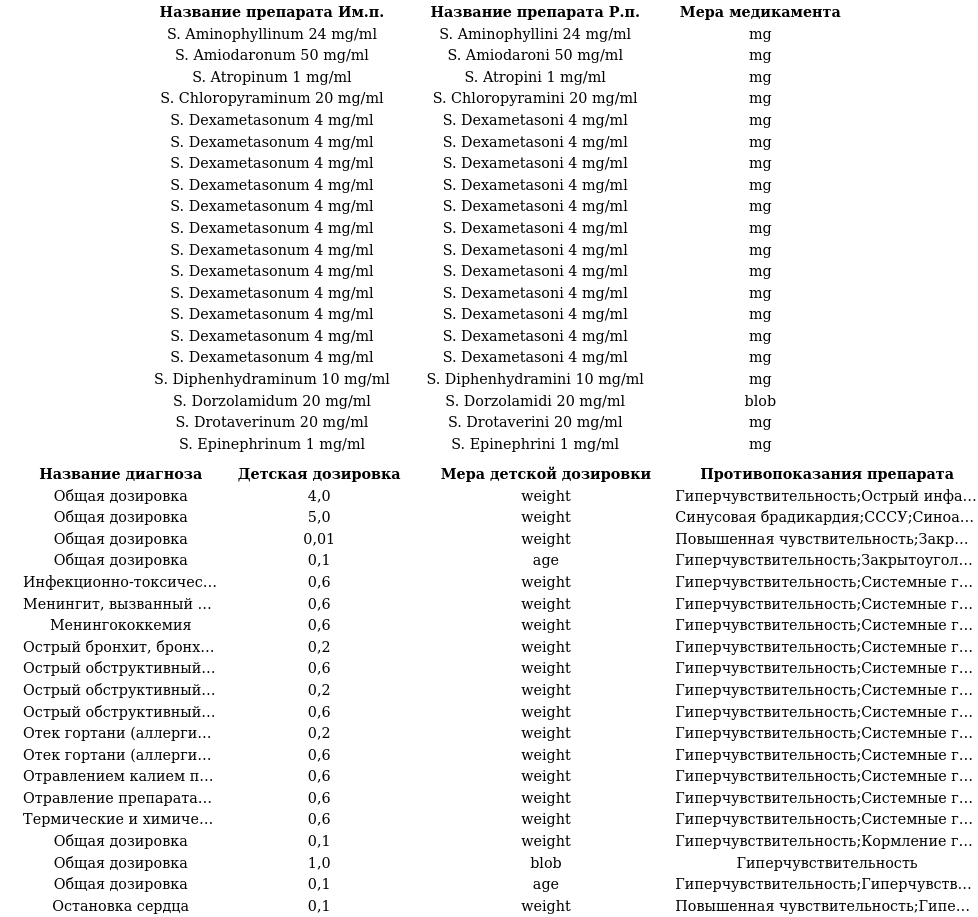
\includegraphics[scale=0.955]{inc/sh_all_ch_med1}
  \caption{Результаты запроса к таблицам медикаментов}
  \label{fig:fig22}
\end{figure}

Все результаты моей деятельности - проектирования, выполнения запросов и их оптимизация, впоследствии передаются на бэкенд. На рисунке~\ref{fig:fig23} представлен JSON формат по отображению всех медикаментов со взрослыми и детскими дозировками из данных, полученных при обращении к БД.

\begin{figure}
  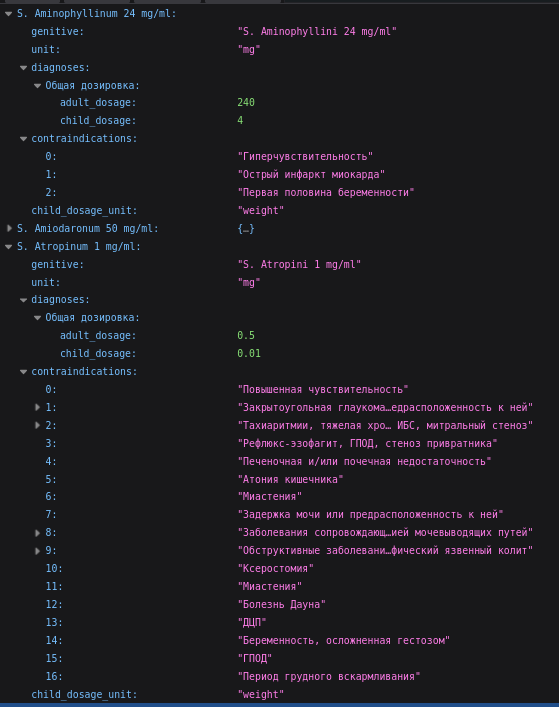
\includegraphics[scale=1.1]{inc/json_sh_all_med1}
  \caption{JSON формат данных, полученных при обращении бэкенда к таблицам медикаментов}
  \label{fig:fig23}
\end{figure}

На рисунке~\ref{fig:fig24} представлен SQL запрос к таблицам заболеваний, представленных на рисунке~\ref{fig:fig06}.

\begin{figure}
  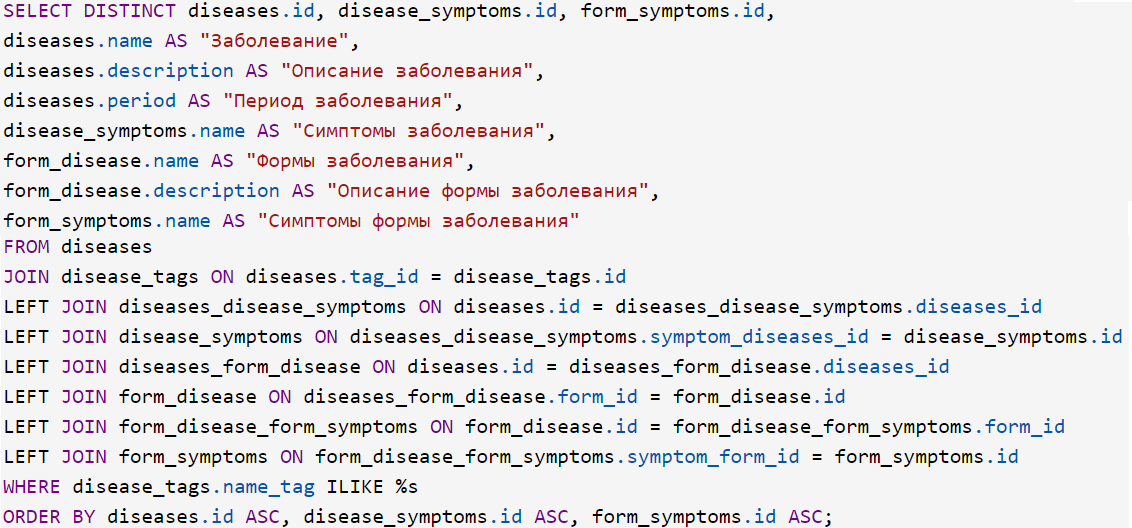
\includegraphics[scale=0.82]{inc/json_sh_dis_part_name}
  \caption{SQL запрос по части названия заболевания}
  \label{fig:fig24}
\end{figure}

На рисунке~\ref{fig:fig25} представлен вывод SQL запроса с рисунка~\ref{fig:fig24}.

\begin{figure}
  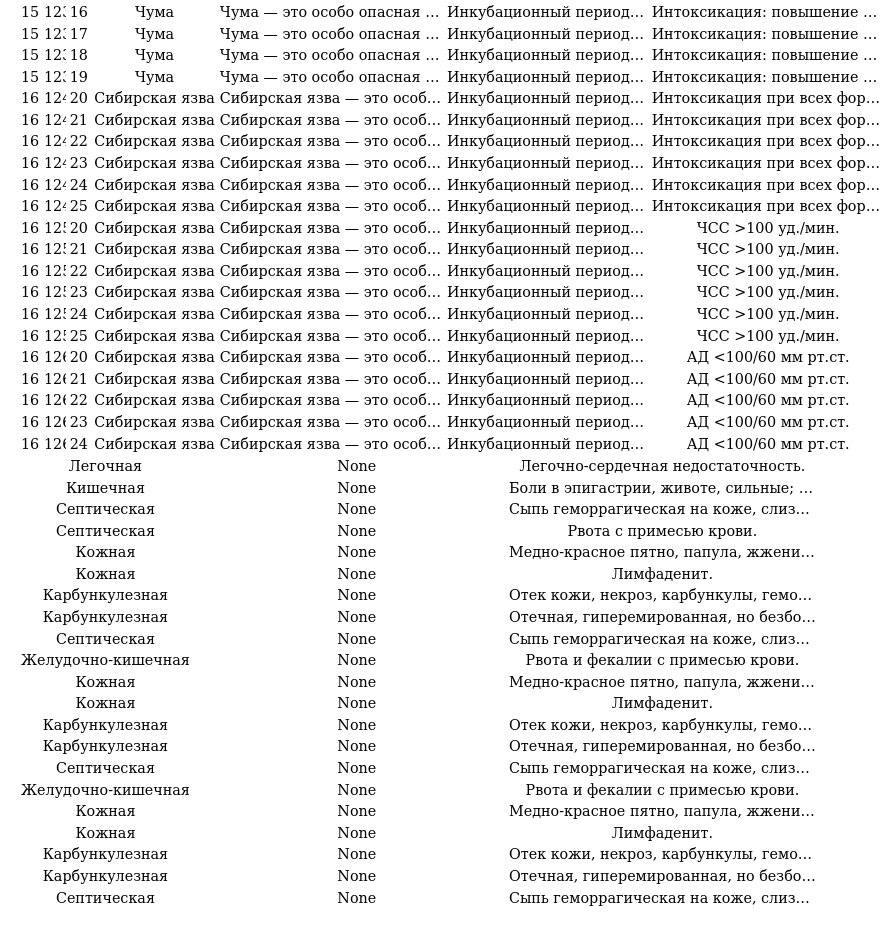
\includegraphics[scale=0.87]{inc/json_sh_dis_part_name1}
  \caption{Результаты запроса к таблицам заболеваний}
  \label{fig:fig25}
\end{figure}

На рисунке~\ref{fig:fig26} представлен JSON формат по отображению всех заболеваний из данных, полученных при обращении к БД.

\begin{figure}
  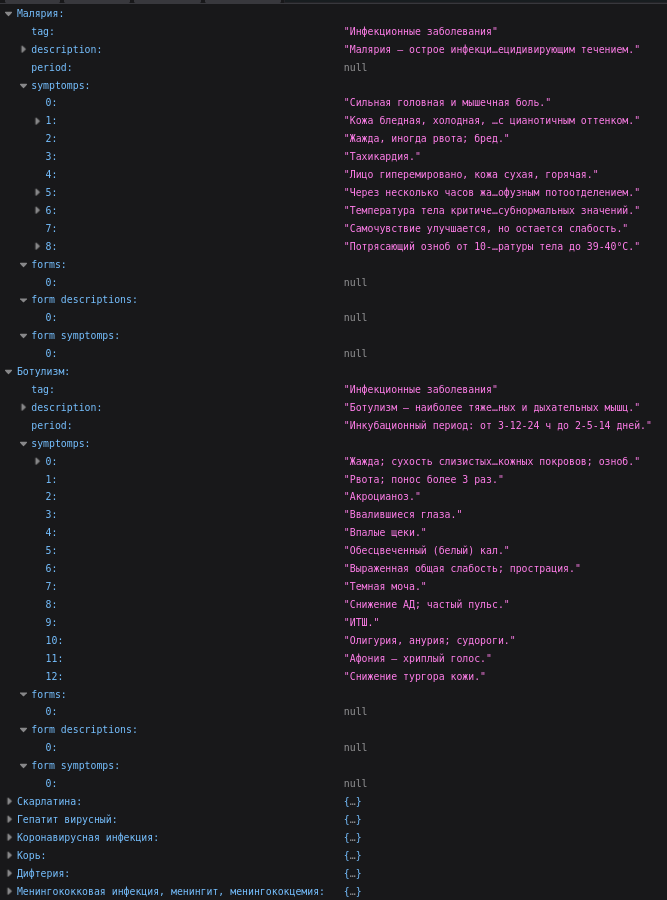
\includegraphics[scale=0.92]{inc/json_sh_dis_part_name2}
  \caption{JSON формат данных, полученных при обращении бэкенда к таблицам заболеваний}
  \label{fig:fig26}
\end{figure}

На рисунках выше были приведены примеры запросов и полученные данные основных таблиц: заболевания, диагнозы и медикаменты. Но кроме основных, еще имеются вспомогательные таблицы дифференциальной диагностики, которые носят информативно-вспомогательный характер.

На рисунке~\ref{fig:fig27} представлены SQL запросы к таблицам дифференциальной диагностики для корректного взаимодействия с бэкендом.

\begin{figure}
  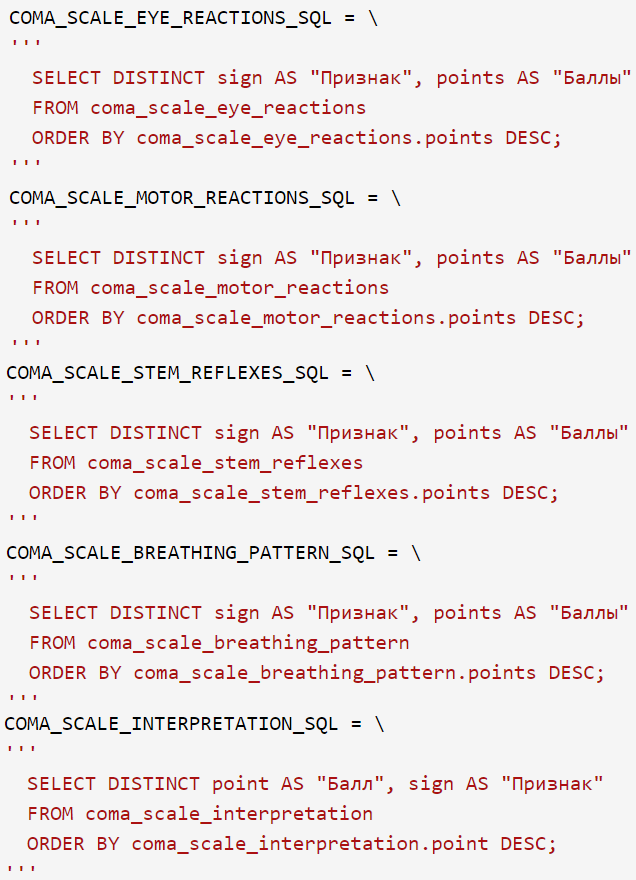
\includegraphics[scale=1.1]{inc/sh_one_table}
  \caption{SQL запросы к таблицам дифференциальной диагностики}
  \label{fig:fig27}
\end{figure}

На рисунке~\ref{fig:fig28} представлен JSON формат таблиц дифференциальной диагностики из данных, полученных при обращении бэкенда к БД.

\begin{figure}
  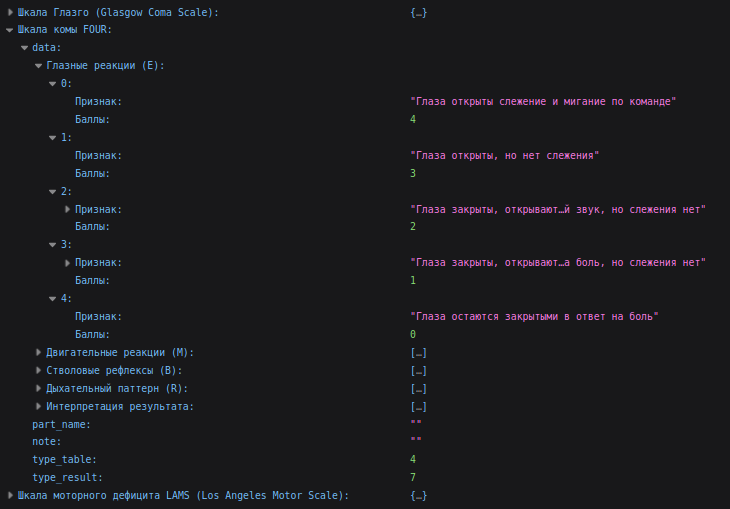
\includegraphics[scale=0.83]{inc/sh_one_table1}
  \caption{JSON формат данных, полученных при обращении к таблицам заболеваний}
  \label{fig:fig28}
\end{figure}

На рисунке~\ref{fig:fig29} представлен JSON формат всех таблиц дифференциальной диагностики.

\begin{figure}
  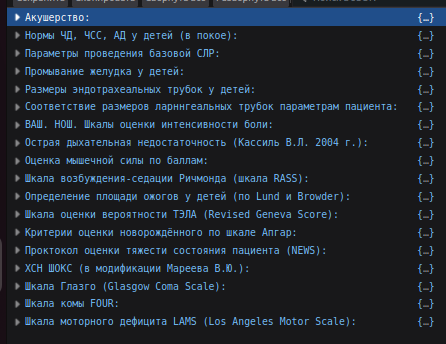
\includegraphics[scale=1]{inc/sh_all_tables}
  \caption{Таблицы дифференциальной диагностики}
  \label{fig:fig29}
\end{figure}



\bigbreak
\textbf{Выводы по разделу}
\bigbreak

Тестирование базы данных является критически важным этапом в разработке и поддержке приложений, использующих базы данных. Тестирование базы данных позволяет убедиться в корректности и надежности ее работы, а также обеспечить защиту от ошибок и нарушений безопасности.

Использование различных методов и инструментов позволяет выявить проблемы в базе данных еще на ранних стадиях и устранить их до того, как они приведут к серьезным проблемам в работе приложения. Кроме того, тестирование базы данных помогает повысить уровень доверия пользователей к приложению и защитить данные от нарушений и утечек. В целом, проведение тестирования базы данных является критически важным для обеспечения надежности, безопасности и производительности приложений.
    
    \conclusion

В выпускной квалификационной работе бакалавра были рассмотрены особенности внедрения цифровых технологий в работу отделения неотложной медицинской помощи, а также разработана система электронных медицинских карт на базе PostgreSQL, которая позволяет улучшить качество и эффективность работы скорой медицинской помощи.

Был проведен анализ системы медицинских карт и баз данных на языке PostgreSQL, а также их применение в работе скорой медицинской помощи. Также были рассмотрены вопросы обеспечения безопасности хранения медицинских данных и конфиденциальности пациентов при использовании электронных медицинских карт.

Помимо БД, имеющей нормализованную структуру, была проведена работа по её защите. Защита строилась как внутренними механизмами и функционалом PostgreSQL Server, так и посредством использования встроенной опциональности ОС.

В работе использовался PostgreSQL для хранения всех возможных данных пациентов. Это позволило создать систему, которая может автоматизировать процесс сбора и обработки данных, а также обеспечивать быстрый и безопасный доступ к истории болезней и личным данным пациентов.

БД спроектирована и защищена, поэтому её можно вводить в эксплуатирование. По желанию в неё можно добавить дополнительный функционал, состоящий из: представлений, индексов, функций и процедур. Все эти объекты БД может настроить администратор или лицо, обслуживающее её, по желанию сотрудников, работающих с ней. Основной функционал и защита были выполнены исходя из целей, а именно:

\begin{itemize}
    \item изучения особенностей предметной области;
    \item проектирования логических и физических моделей данных;
    \item разработки структуры базы данных;
    \item нормализация данных;
    \item определения и настройки защитных мер;
    \item обеспечения конфиденциальности хранения персональных данных;
    \item проведение тестирования, оптимизации запросов и структуры базы данных.
\end{itemize} % Заключение

    \printbibliography % Список литературы

    \appendix % Приложения
    \appendixsection{QR-код с ссылкой на GitHub репозиторий}

На рисунке ~\ref{fig:a1} представлен QR-код с ссылкой на GitHub репозиторий со всеми файлами, ER-диаграммами, SQL-кодом разработанной базы данных и всего необходимого функционала.

\begin{figure}
    
\includegraphics[width=10cm]{inc/QR-code}
    \caption{QR-код с ссылкой на GitHub репозиторий}
    \label{fig:a1}
\end{figure}

%    \appendixsection{Приложение с листингом}

Рисунок~\ref{src:src3} с листингом в приложении.

\begin{figure}
\lstinputlisting[language=C++]{inc/example.cpp}
\caption{Пример использования листинга}
\label{src:src3}
\end{figure}
\end{document}